% fix bugs: fixes already in kernel now
%\RequirePackage{fixltx2e}


\documentclass[10pt]{report}

% encoding of tex-file
\usepackage[utf8x]{inputenc}

% for propper Umlaute
\usepackage[T1]{fontenc}

% proper hyphenation
\usepackage[english]{babel}

% better i18n Postscript version of Knuth's cm fonts, better than cm-super
\usepackage{lmodern}

% Mathematics
\usepackage{mathtools} % extension and fixes of/in amsmath
\usepackage{amssymb} % provides symbols, loads amsfonts
\usepackage{amsthm} % provides theorem environment
%\usepackage{nicefrac} % better slash fracs in inline

% For including figures, rotating or scaling text (dont use file extension)
\usepackage{graphicx}

% rotate figures
\usepackage{rotating}

% LS-Lab auxiliary math commands
\usepackage{math}

% LS-Lab logic commands: includes lcalculus, lmeta, lsemantics, lsyntax
\usepackage[
    varterms, sigmaterms, septerms,
    substopinline,
    modifopinline, % arrow notation for \imodif in semantics
    longinterpret,
    %bracketinterpret,%
    %fixformat,%
    sidenotecalculus,%
    %silentconst,%
    longseqcontext%
    ]{logic}

% LS-Lab differential dynamic logic commands
\usepackage[
    %bracketmodalinterpret,% use [[]] for semantics
    bracketmodalinterpret,%
    fixformat,%
    %silentconst,% don't show `const' and `algebra'
    precisenames%
    ]{dL}


% own symbol definitions
%
% Math Environements
%
% italic text
\newtheorem{theorem}{Theorem}[chapter]
\newtheorem{corollary}[theorem]{Corollary}
\newtheorem{proposition}[theorem]{Proposition}
\newtheorem{lemma}[theorem]{Lemma}
% normal text
\theoremstyle{definition}
\newtheorem{definition}[theorem]{Definition}
\newtheorem{example}[theorem]{Example}

%
% General Mathematics
%
% natural numbers
\newcommand{\N}{\mathbb{N}}
% real numbers
\newcommand{\R}{\mathbb{R}}
% integer range
\newcommand{\range}[2]{#1,\ldots,#2}
% functions: f\from\R\to\R
\newcommand*{\from}{\colon}
% define as
% FIXME: define "def" properly
%\newcommand{\defeq}{\,\stackrel{\text{def}}{=}\,}
% defined by
\newcommand\logeq{\mathrel{\vcentcolon\Longleftrightarrow}}
% norm
%\DeclarePairedDelimiter{\abs}{\lvert}{\rvert}
\DeclarePairedDelimiter{\nnorm}{\lVert}{\rVert}
\DeclarePairedDelimiter{\supnorm}{\lVert}{\rVert_{\text{\scriptsize{sup}}}}

% exponential function
\newcommand{\e}[1]{\text{e}^{#1}}

%
% Analysis
%
% derivative: Lagrange style
%\newcommand{\D}[1]{#1'} % ' defined in latex and is same as \prime
% derivative: Leibniz style
\renewcommand{\DD}[2]{\frac{\text{d} #1}{\text{d} #2}}
% differential in integral
\newcommand{\dx}[1][x]{\text{d}#1}

\newcommand{\continuouspws}[3][]{\ensuremath{C^{#1}_\text{pw}\ifthenelse{\equal{#2}{}}{}{\ifthenelse{\equal{#3}{}}{(#2)}{(#2,#3)}}}}

%
% Delay Differential Equation
%
% definition domain of right hand side
\newcommand{\deff}{\R\times\R^n\times\R^n}

%
% Differential Dynamic Logic
%
% ddL
\newcommand{\ddL}{\textsf{dd{\kern-0.1em}$\mathcal{L}$ }}
\newcommand{\signature}{\Sigma}
\newcommand{\varsymbols}{V}
\newcommand{\terms}{\lterms{\signature}{\varsymbols}}
\newcommand{\FOLformulas}{\lformulas[\FOL]{\signature}{\varsymbols}}
\newcommand{\FOL}{\text{FOL}}
\newcommand{\FOLR}{\FOL$_\R$}
% FIXME: use \mathcal{M}
\newcommand{\model}{M}
\newcommand{\interpret}[1][]{\ifthenelse{\equal{#1}{}}{I}{I(#1)}}
\newcommand{\universe}{D_{\model}}
\newcommand{\assignment}{\nu}
\newcommand{\ireachability}[2]{\rho\left(#2\right)}
%
% Delay Differential Dynamic Logic
%
\renewcommand{\ivr}{\chi}
\newcommand{\csfml}{\chi}

% formula of first-order real arithmetic
\newcommand{\asfmlfolR}{\chi}

% propositions
\newcommand{\asprop}{p}
\newcommand{\bsprop}{q}

% sets of formulas
\newcommand{\asfmls}{\Gamma}
\newcommand{\bsfmls}{\Delta}
\newcommand{\csfmls}{\Theta}

% states
\newcommand{\states}{\mathcal{S}}
\newcommand{\asstate}{\nu}
\newcommand{\bsstate}{\omega}
\newcommand{\csstate}{\mu}

\newcommand{\delayinterval}[1][T]{[-#1,0]}

\newcommand{\diffvars}{\D{\allvars}}
\newcommand{\delayedvars}{\mathcal{V}_\tau}

\newcommand{\statespace}[1][T]{\continuouspws[0]{\delayinterval[#1]}{\R^n}}
%\newcommand{\xtau}[1][]{\ifthenelse{\equal{#1}{}}{x[\tau]}{x[#1]}}
\newcommand{\x}[1][]{x[#1]}
\newcommand{\xtau}[1][\tau]{x[-#1]}
\newcommand{\Dxtau}[1][\tau]{\D{x}[-#1]}
\newcommand{\holdssince}[3][s]{\lforall{#1\in\delayinterval[#2]}{\left(#3\right)}}

\newcommand{\xbartau}{\bar{x}_{\tau}}
\newcommand{\xbartaut}[1]{\bar{x}_{\tau,#1}}


\newcommand{\IFOL}{\interpretation[
    algebra=\model,
    %const=I,
    %assign=\assignment,
    % state=\nu,
    universe=\universe
    ]}

\newcommand{\IML}{\interpretation[
    algebra=\model,
    %const=I,
    %assign=\assignment,
    state=\nu,
    worlds=W,
    access=R,
    universe=\universe
    ]}

\newcommand{\IddL}{\dLint[
    const=I,
    state=\nu,
    access=\rho
    ]}
%%%%%%%%%%%%%%%%%%%%%%%%%%%%%%%%%%%%%%%%%%%%%%%%%%%%%%%%%%%%%%%%%%%%%%%%%%%


\begin{document}

\title{Delay Hybrid Systems}

\author{Lorenz Sahlmann\\ École Polytechnique\\ Carnegie Mellon University}
\date{\today}

\maketitle

\begin{abstract}
    In this work we extend Differential Dynamic Logic with Delay Differential Equations.

    This requires an extension of the syntax, a (partially) redefinition of the semantics and the introduction of additional axioms and proof rules.

    This results in a superset of \dL which we call \textbf{Delay Differential Dynamic Logic}.
\end{abstract}

%\chapter{Introduction}


\chapter{Delay Differential Equations}

special case of more general functional differential equations (FDEs)

often arise in automatic control
controller montitor state of systems
control decision to adjust state
delay between observation and control action

depends on earlier values
depends on current value and past
need to specify in initial condition
at least for the time of longest delay

delays can be both stabilizing and destabilizing
stability in many application an important property

Examples
epidemics
traffic flow
vibrations, chattering
-> ref in \cite{Falbo06FDEs}

methods to solve analytically \cite{Falbo06FDEs}

\section{Piecewise Continuous Functions}
    \label{sec:piecewise-continuous-functions}
    
    The following definition is motivated by capturing the character evolution arising from hybrid systems. We will see that we can consider such to be piecewise continuous.

    % \begin{definition}[Piecewise Continuous]\label{def:piecewise-continuous}
    %     Let $D=[a,b]\subseteq\R$ be a closed interval (this includes the cases when $a=-\infty$ or $b=\infty$, or both). The mapping $x:D\rightarrow\R^n$ is called \emph{piecewise continuous} if and only if there is a finite partition $\{t_i:i=\range{0}{m}\}$ of $D$ (i.e.\ $a=t_0<t_1<\ldots<t_m=b$) such that $x$ is continuous on each interval piece $[t_i,t_{i+1})$ for all $i=\range{0}{m-1}$ and the left sided limits
    %     \begin{equation}
    %         \lim_{\substack{t\upto t_{i+1}\\ t\in[t_i,t_{i+1})}} x(t)
    %     \end{equation}
    %     exist. Hence $x(b)$ can be an isolated point and this right interval limit $b$ is the only spot where such is allowed.

    %     We denote by $\Cnpw[0]{D}{\R^n}$ the set of \emph{piecewise continuous functions} on the compact interval $D$ (this excludes the cases with $\pm\infty$), mapping to $\R^n$.
    % \end{definition}

    \begin{definition}[Piecewise Continuously Differentiable]\label{def:pw-cont-diff}
        % FIXME: find better word for 'partition'. partition?
        Let $D=[a,b]\subseteq\R$ be a closed interval (this includes the cases when $a=-\infty$ or $b=\infty$, or both). The mapping $x:D\rightarrow\R^n$ is called $n$-times \emph{piecewise continuously differentiable} if and only if there is a finite partition (ordered set) $\{t_i:i=\range{0}{m}\}$ of $D$ (i.e.\ $a=t_0<t_1<\ldots<t_m=b$) such that $x$ is $n$-times continuously differentiable on each interval piece $(t_i,t_{i+1})$ with continuable derivatives on $\compactum{t_i}{t_{i+1}}$ right continuous with left limits.
        \emph{càdlàg} (``continue à droite, limite à gauche'')
        knots

        This means, for all $i=\range{0}{m-1}$ and for all $k=\range{0}{n}$ exist the left sided limits
        \begin{equation}
            \lim_{\substack{t\upto t_{i+1}\\ t\in(t_i,t_{i+1})}} \D[k]{x}(t)
        \end{equation}
        as well as the right sided limits
        \begin{equation}
            \lim_{\substack{t\downto t_{i}\\ t\in(t_i,t_{i+1})}} \D[k]{x}(t) =: \D[k]{x}(t_i)
        \end{equation}
        which are supposed to coincide with the value of $\D[k]{x}$ at $t_i$.
        Hence $x(b)$ can be an isolated point and this right interval limit $b$ is the only spot where such is allowed.
        In the case $n=0$, we say $x$ is \emph{piecewise continuous}.

        We denote by $\Cnpw[n]{D}{\R^n}$ the set of \emph{$n$-times piecewise continuously differentiable functions} on the compact interval $D$ (this excludes the cases with $\pm\infty$), mapping to $\R^n$, and respectively, by $\Cnpw[0]{D}{\R^n}$ the \emph{piecewise continuous functions}.
    \end{definition}

    % TODO: sup-norm for pw

    \begin{lemma}
        chain of continuous and piecewise-continuous is again piecewise-continuous with same partition
    \end{lemma}

    \begin{lemma}[]\label{lm:pc-integrable}
        A \emph{piecewise continuous function}, as defined in Definition~\ref{def:pw-cont-diff} is (Riemann) integrable.
    \end{lemma}
    \begin{proof}
        See standard analysis literature, such as \cite{Rudin76PrinciplesAnalysis} (Theorem~6.10) or \cite{Gathmann12GDM} (Example~11.16b).
        % ObdA: one subint with jump at end
    \end{proof}

    The following lemma generalizes the fundamental theorem of calculus to piecewise continuous derivatives.

    \begin{lemma}[]\label{lm:pc-hauptsatz}
        Let $F\in\Cn[0]{\compactum{a}{b}}{} \cap \Cnpw[1]{\compactum{a}{b}}{}$ with the partition $\partition{a=t_0}{t_m=b}$ and piecewise derivative $f$.
        %of $\compactum{a}{b}\subset\R$. 
        For all $t\in\compactum{a}{b}$ it holds
        \begin{equation*}
            F(t)-F(a) = \integral{a}{t} f(s)\dx[s]
            %\sum_{i=0}^k\int\limits_{t_i}^{t_{i+1}}f(t)\dx[t] + \int\limits_{t_k}^s f(t)\dx[t]
        \end{equation*}
        %where $t_k\leq s < t_{k+1}$.
        % FIXME: what about a=-inf or b=inf?
    \end{lemma}
    \begin{proof}
        On each interval $\compactum{t_{i-1}}{t_i}$ of the partition, $f$ is piecewise continuous and hence integrable.

        For all $\zeta\in\open{t_{i-1}}{t_i}$ is $F$ differentiable on $\compactum{t_{i-1}}{\zeta}$ with $\D{F}=f$.
        By the fundamental theorem of calculus (cf.\ standard analysis literature, e.g.~\cite{Gathmann12GDM,Rudin76PrinciplesAnalysis}), it follows
        \begin{equation*}
            \denseintegral{t_{i-1}}{\zeta} f(s)\dx[s] = F(\zeta)-F(t_{i-1})
        \end{equation*}
        and by the continuity of $F$ that
        \begin{equation*}
            \denseintegral{t_{i-1}}{t_i} f(s)\dx[s]
            = \lim_{\zeta\to t_i}\denseintegral{t_{i-1}}{\zeta} f(s)\dx[s]
            = \lim_{\zeta\to t_i} F(\zeta)-F(t_{i-1})
            = F(t_i)-F(t_{i-1})
        \end{equation*}
        For any $t\in\compactum{a}{b}$, there is a $k\in\set{\range{1}{m}}$ such that $t\in\closedopen{t_{k-1}}{t_k}$ (in the case $t=b$, set $k=m$), summation over $i=\range{1}{k}$ yields the telescoping series
        \begin{equation*}
            F(t)-F(a) = \sum_{i=1}^{k} \denseintegral{t_{i-1}}{t_i} f(s)\dx[s] + \integral{t_j}{t} f(s)\dx[s]
        \end{equation*}
        which is by the additivity of the integral
        \begin{equation*}
            F(t)-F(a) = \integral{a}{t} f(s)\dx[s]
        \end{equation*}
    \end{proof}

% \begin{figure*}[h]\centering
%     \begin{subfigure}[t]{0.5\textwidth}\centering
%         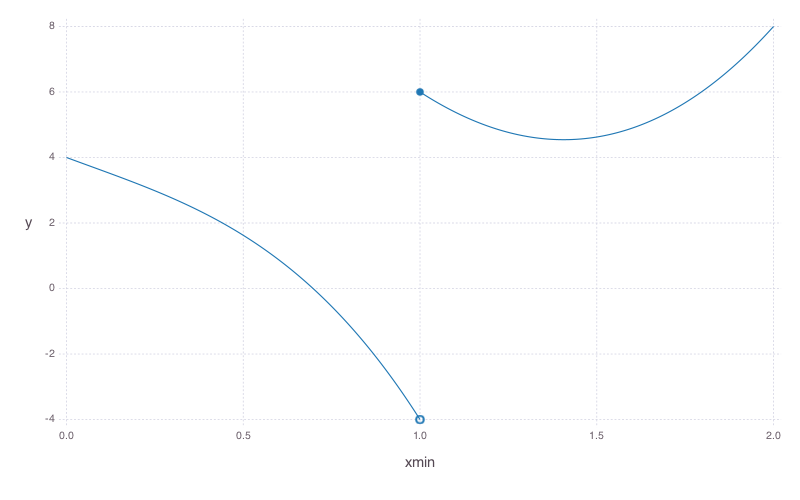
\includegraphics[width=\textwidth]{figures/allowed.png}
%         \caption{Admissible piecewise continuous function.}
%         \label{fig:allowed}
%     \end{subfigure}
%     \begin{subfigure}[t]{0.5\textwidth}\centering
%         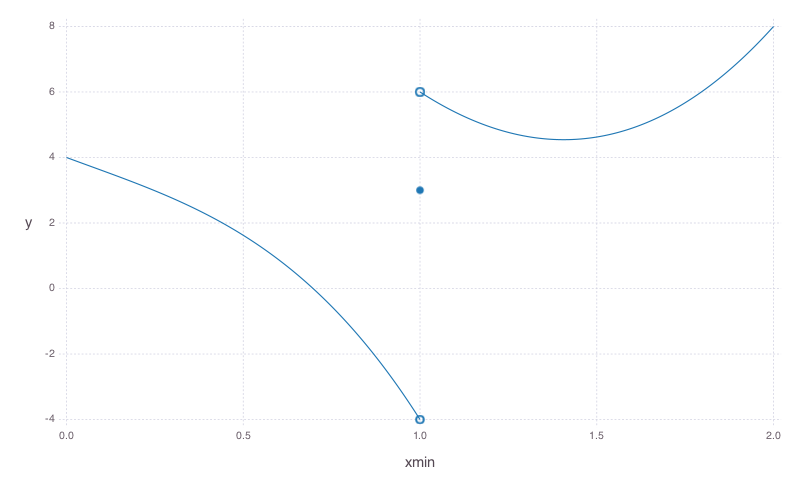
\includegraphics[width=\textwidth]{figures/not-allowed.png}
% 	    \caption{Not allowed!}
% 	    \label{fig:not-allowed}
%     \end{subfigure}
%     \caption{Examples to Definition \ref{definition-piecewise-continuous}.}
% \end{figure*}


\section{Definition DDE}
    \label{sec:definition-dde}
    % TODO: multiple fixed, discrete, bounded delay

    % TODO: also, but not here: state-dependent delay, distributed delay

    \cite{Roussel04DDEs}

    \begin{definition}[Delay Differential Equation]\label{def:dde}
        Let $f\from\deff\to\R^n$ and time delays $0<\tau_1<\ldots<\tau_k$ $\tau_j > 0$ for $j=\range{1}{k}$. Put $\taumax\defeq\tau_k\max_j\set{\tau_j}$ and $\taumin\defeq\tau_1$.

        A functional equation of the form
        \begin{equation}\label{eq:dde}
            \D{x}(t) = f(t,x(t),x(t-\tau_1),\ldots,x(t-\tau_k))
        \end{equation}
        is called (first order) \emph{delay differential equation} (DDE) with \emph{multiple constant, discrete delays $\tau_j$}.
        It is \emph{autonomous} if its right hand side $f$ is time independent and \emph{pure} if the right hand side only depends on $x(t-\tau_i)$ and not on $x(t)$.

        A DDE can be equipped with an \emph{initial condition} $x_{\tzero}$. It specifies the state, i.e.\ the values of $x$ on $[\tzero-\taumax, \tzero]$ on which the right hand side depends.
        Such a pair is called \emph{initial value problem (IVP)}:
        \begin{equation}\label{eq:ivp}
            \begin{cases}
                \D{x}(t) = f(t,x(t),x(t-\tau_1),\ldots,x(t-\tau_k)) & \text{for } t\geq\tzero\\
                x(t) = x_{\tzero}(t) & \text{for } t\in [\tzero-\taumax,\tzero]
            \end{cases}
        \end{equation}
    \end{definition}

    % Since we only consider autonomous DDEs, we can without loss of generality restrict to the case of initial time $t_0=0$.

    % The definition of a DDE can be extended to multiple constant discrete delays. For simplicity, we restrict here to a single delay.


\section{Definition of Solution}
    \label{sec:definition-of-solution}

    \begin{definition}[Solution of DDE]\label{def:solution-dde}
        A function $x\from\compactum{\tzero-\taumax}{\tzero+T}\to\R^n$ is called \emph{(local) solution} of the initial value problem~\eqref{eq:ivp}, if and only if
        $x$ is continuous and piecewise continuously differentiable on $\compactum{\tzero}{\tzero+T}$ (in the sense of Def.~\ref{def:piecewise-continuous}) with partition $\Delta$.
        This means, when $\Delta=\partition{\tzero=t_0}{t_m=\tzero+T}$, $x$ is continuously differentiable on each interval $(t_i,t_{i+1})$
        %there exists a $T>0$ such that
        % FIXME: local solution is on a single subdiv int only -> cont diffable
        %$\restrict{x}{(t_i,t_{i+1})}\in \Cn[1]{\compactum{\tzero}{\tzero+T}}{\R^n}$ with
        with
        \begin{equation*}
            \D{x}(t) = f(t,x(t),x(t-\tau_1),\ldots,x(t-\tau_k))
        \end{equation*}
        for all $t\in (\tzero,\tzero+T)$ and in $t=t_i$, it holds
        % TODO: for the right-hand derivative?
        % cf ODE sol
        \begin{equation*}
            \lim_{s\downto t_i}\D{x}(s) = f(t_i,x(t_i),x(t_i-\tau_1),\ldots,x(t_i-\tau_k))
        \end{equation*}
        and $x$ obeys the initial condition:
        \begin{equation*}
            x(t) = x_{\tzero}(t) \quad\text{for } t\in [\tzero-\taumax,\tzero].
        \end{equation*}
        % FIXME: global solution should allow knicks
        If the function $x$ is a solution for all $T>0$, it is called \emph{global}.

        %TODO: differentiable in right rand point? need not derivative in right hand point
        in knots: right sided derivative
        %TODO: Fortsetzbarkeit For example initial condition has jump, this point is limit for local solution.
    \end{definition}

\cite{Roussel04DDEs}
solution of equation is operator mapping from functions on $\compactum{t-\taumax}{t}$ to functions on $\compactum{t}{t+\taumax}$
then solution of initial value problem sequence of these functions
derivative not necessarily continuous at knots

% \begin{figure}[h]\centering
%     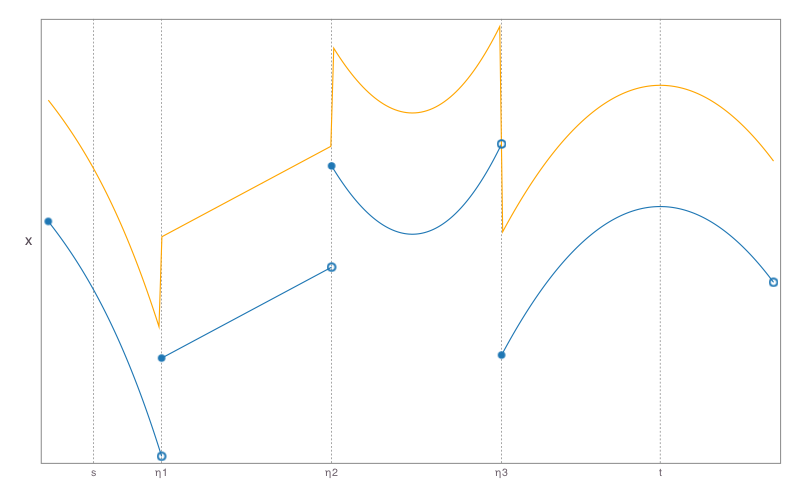
\includegraphics[width=\textwidth]{figures/multiple.png}
% 	\caption{Illustration of proof to Lemma \ref{lemma-continuity}}
% 	\label{fig:not-allowed}
% \end{figure}

% FIXME: This lemma is wrong. Show instead integrability of f(t,x_t)
\begin{lemma}
    \label{lemma-continuity}

    % Let $x:[\tzero-\tau,\tzero+T] \rightarrow \R^n$ be piecewise continuous (as in Definition \ref{definition-piecewise-continuous}) with the partition $\{t_0,\ldots,t_k\}$, i.e. there are $k$ subintervals.
    %
    % Then $t \mapsto x_t = x(t+\theta)$, where $\theta\in[-\tau,0]$, is a piecewise continuous mapping from $[\tzero,\tzero+T]$ into $\statespace[\tau]$.
\end{lemma}

\begin{proof}
    % $x$ is piecewise continuous and hence uniformly piecewise continuous on the compact interval $I=[\tzero-\tau,\tzero+T]$.
    % i.e. uniformely continuous on each subinterval with stetiger Fortsetzung in right side.
    % \begin{equation}
    %     \forall\epsilon >0 \exists\delta_i >0 \forall t,s\in I_i: \quad \abs{t-s}<\delta_i \Rightarrow \nnorm{x(t)-x(s)}<\epsilon
    % \end{equation}
    % Let $\epsilon > 0$. $x|_{[t_i,t_{i+1}]}$ (with stetiger fortsetzung in right interval limit) is uniformly continuous, i.e. there is a $\delta_i > 0$ (for the given $\epsilon$), such that $\forall\,t, s \in [t_i,t_{i+1}]$ holds
    % % TODO: can use \leq ?
    % \begin{equation}
    %     \abs{t-s} < \delta_i \Rightarrow \nnorm{x(t)-x(s)} < \epsilon
    % \end{equation}
    %
    % Among the given $\delta_i$, choose the smallest as $\delta = \min_i \delta_i$.
    %
    % For any $i$ and $s,t\in [t_i,t_{i+1})\subset [\tzero,\tzero+T]$ with $\abs{t-s}<\delta$, it holds
    % \begin{equation}
    %     \supnorm{x_t - x_s} = \sup_{\theta\in [-\tau,0]}\nnorm{x(t+\theta) - x(s+\theta)} < \epsilon
    % \end{equation}
    % since $t+\theta, s+\theta \in I$
    % Hence $t \mapsto x_t$ is uniformely continuous on $[t_i,t_{i+1})$.
\end{proof}


\section{Method of Steps}
    \label{sec:method-of-steps}
    
    See \cite{Falbo06FDEs}
    by restricting the IVP onto an interval
    actually have an ODE IVP
    convert DDE into a ODE on a certain interval, by plugging the given initial condition into the delay differential equation, eliminating the explicit dependance on the past
    can be repeated on next interval by inserting the previously computed solution instead of the initial condition

    for $t\in [0,\tau]$, $x$ must satisfy the following ordinary initial value problem obtained by plugging the initial function into equation (??). For suitable $f$ and $x_0$, the existence (and uniqueness) of a solution on $[0,\tau]$ is guaranteed by ODE theory (\ldots{} or Picard-Lindelöf theorems).

    This procedure can then be applied repeatedly to extend the obtained solution by steps of length $\tau$.





\section{Existence and Uniqueness of Solutions}
    \label{solutions-existence-uniqueness}

    cannot have more than one solution
    under certain conditions, there is such 

    will consider rhs cont and lip
    $f$ Lipschitz with piecewise continuous initial function have existence and uniqueness ???? smoothing

    \begin{definition}[Lipschitz Continuity]\label{def:lipschitz}
        % similar to \cite{pruesswilke10GewDiffGl,Smith10IntroDDE}
        % FIXME: dont I need xtau in right side ??? 
        A function $f\from\deff\to\R^n$ is called \emph{(locally) Lipschitz continuous} (in its $i$-th argument) if and only if for all $a,b\in\R$ and $M>0$ there is a $L>0$ such that
        \begin{equation*}
            % TODO: is L(\nnorm*{x-x}+\nnorm*{y-y}) better? is equiv, with different L
            % FIXME: or just say Lipschitz continuous with respect to two other arguments, once for x once for y -> compare proof
            \nnorm*{f(t,x_1,\ldots,x_i,\ldots,x_k) - f(t,x_1,\ldots,y_i,\ldots,x_k)} \leq L\nnorm*{x_i - y_i}
        \end{equation*}
        for all $t\in [a,b]$ and $x_j,y_i\in\R^n$ with $\nnorm{x_j},\nnorm{y_i},\leq M$.
    \end{definition}

    \begin{lemma}\label{lm:bounded-lipschitz}
        Let $f\from\deff\to\R^n$ be continuous and Lipschitz continuous in all but its first argument.

        For any given compact interval $\compactum{a}{b}$ and $M>0$ there exists a bound $K>0$ such that
        \begin{equation}
            \nnorm{f(t,x_1,\ldots,x_k)}\leq K
        \end{equation}
        for all $t\in\compactum{a}{b}$ and $x_j\in\R^n$ with $\nnorm{x_j}\leq M$.
    \end{lemma}
    \begin{proof}
        Let $L_i$ be the Lipschitz constant for the $i$-th argument of $f$ on the given $\compactum{a}{b}$ and $M$. Set $L\eqdef\max_i\set{L_i}$. Then
        \begin{multline*}
            \nnorm{f(t,x_1,\ldots,x_k)} \leq \nnorm{f(t,x_1,\ldots,x_k) - f(t,0,\ldots,0)} + \nnorm{f(t,0,\ldots,0)}\\
            \leq L_i\nnorm{x_i-0} + \nnorm{f(t,0,\ldots,0)} \leq LM+P = K
        \end{multline*}
        for $t\in\compactum{a}{b}$ and $x_j\in\R^n$ with $\nnorm{x_j}\leq M$. We used the continuity of $f$ on the compact set $\compactum{a}{b}$ for the existence of
        \begin{equation*}
            P = \max_{s\in\compactum{a}{b}}\nnorm{f(s,0,\ldots,0)}
        \end{equation*}
    \end{proof}

    \begin{lemma}\label{lm:integral-equation}
        %TODO: compare with ODE lecture notes
        Finding a solution of the initial value problem~\eqref{eq:ivp} is equivalent to solving the integral equation
        \begin{equation*}\label{eq:integral-equation}
            \begin{cases}
                x(t) = x_{\tzero}(\tzero) + \integral{\tzero}{t} f(s,x(s),x(s-\tau_1),\ldots,x(s-\tau_k))\dx[s] & \text{for } t\geq\tzero\\
                x(t) = x_{\tzero}(t) & \text{for } t\in [\tzero-\taumax,\tzero]
            \end{cases}
        \end{equation*}
        where ... (same as for ivp)
        and is continuous in t.
        integral componentwise, f vector valued
    \end{lemma}
    \begin{proof}
        Let $x$ be a solution of the IVP. Thus $x$ is (by definition) piecewise continuous on $\compactum{\tzero-\taumax}{\tzero}$ andcontinuous and piecewise continuous differentiable on $\compactum{\tzero}{\tzero+T}$ with piecewise derivative $f(t,x(t),x(t-\tau_1),\ldots,x(t-\tau_k))$. This chain of a piecewise continuous and continuous function is piecewise continuous and hence by Lemma~\ref{lm:pc-integrable} integrable on $\compactum{\tzero}{\tzero+T}$.

        By Lemma~\ref{lm:pc-hauptsatz} it follows
        \begin{equation*}
            x(t) = x_{\tzero}(\tzero) + \integral{\tzero}{t} f(s,x(s),x(s-\tau_1),\ldots,x(s-\tau_k))\dx[s]
        \end{equation*}
        for $t\geq\tzero$.

        Conversely, let $x$ be a solution of the integral equation~\eqref{eq:integral-equation}.
        By the the fundamental theorem of calculus is $x$ continuous on $\compactum{\tzero}{\tzero+T}$ and differentiable in $t\in\compactum{\tzero}{\tzero+T}$ if $s\mapsto f(s,x(s),x(s-\tau_1),\ldots,x(s-\tau_k))$ is continuous in $s=t$.

         has the partition
        We define a partition of $\compactum{\tzero}{\tzero+T}$ by
        \begin{equation*}
            \mathcal{Z}\defeq\set{\tzero,\tzero+T}\cup\bigcup_{j=1}^{k}\bigcup_{\substack{i=1\\t_i\geq\tau_j}}^{m}\set{t_i-\tau_j}\defeq\partition{\hat{t}_0}{\hat{t}_p}
        \end{equation*}
        If $s\in\open{\hat{t}_{l-1}}{\hat{t}_l}$ then is $s-\tau_j\neq t_i$ for all $j$ and $i$. Hence the mapping $t\mapsto f(t,x(t),x(t-\tau_1),\ldots,x(t-\tau_k))$ is continuous in $t=s$, what implies that $x$ is differentiable in $s$ and that $\D{x}(s)=f(s)$.

        \begin{align*}
            \lim_{s\downto\hat{t}_l} \D{x}(s)
            &= \lim_{s\downto\hat{t}_l} f(s,x(s),x(s-\tau_1),\ldots,x(s-\tau_k))\\
            &= f(\hat{t}_l,x(\hat{t}_l),x(\hat{t}_l-\tau_1),\ldots,x(\hat{t}_l-\tau_k))
        \end{align*}
        by the continuity of $f$ and $\lim_{s\downto\hat{t}_l} x(s-\tau_j) = x(\hat{t}_l-\tau_j)$
        the limits exist
        \begin{equation*}
            \lim_{s\upto\hat{t}_l} \D{x}(s) = \lim_{s\upto\hat{t}_l} f(s,x(s),x(s-\tau_1),\ldots,x(s-\tau_k)) = 
        \end{equation*}
        Obviously, it obeys the initial condition, i.e. $x(t)=x_{\tzero}(t)$ for all $t\in\compactum{\tzero-\tau}{\tzero}$.
        % FIXME: f cont uberall in Voraussetzung?
    \end{proof}

    \begin{theorem}[Existence of unique solution]\label{thm:solution-existence}
        Consider the Delay Differential Equation
    %TODO: do we need global existence or just local?
        \begin{equation}
            \begin{cases}
                \D{x} = f(t,x(t),x(t-\tau)) & \text{for } t\geq\tzero\\
                x(t) = x_\tzero(t-\tzero)   & \text{for } t\in [\tzero-\tau,\tzero]
            \end{cases}
        \end{equation}
        with $f\from\deff\to\R^n$ continuous and satisfying the (local) Lipschitz condition in its second argument (Def.~\ref{def:lipschitz}).

        % where $\nnorm{\cdot}$ denotes the Euclidian norm on $\R^n$ and $\supnorm{\cdot}$ the supremum norm of the Banach space of continuous functions on $[-\tau,0]$.

        Then for each \emph{initial condition} $x_{\tzero}\in\statespace[\tau]$ and start time $\tzero$, there \textbf{exists} a \textbf{unique local solution} of the IVP on a time interval $[\tzero-\tau, \tzero+T]$. The duration $T>0$ depends on the sup-norm and discontinuity points of the initial condition. (?)
        This solution is continuous and piecewise differentiable on $\compactum{\tzero}{\tzero+T}$ with partition $t_i+\tau$.
    \end{theorem}

    The proof is smiliar to the proof of the existence theorem (Theorem 3.7) given in~\cite{Smith10IntroDDE}.
    \begin{proof}
        % FIXME: where sup-norm?
        As a piecewise continuous function, the initial condition can bounded by $M\geq \supnorm{x_\tzero}$ on $\delayinterval[-\tau]$.
        
        % FIXME: do I need t_0+tau or is just \tau okay? do I need x not to be pw, just cont in proof?
        If $\set{\range{-\tau=t_0}{t_k=0}}$ is the partition of $x_{\tzero}$, we choose $T=\min\set{t_0+\tau,\frac{M}{K}}$.
        
        % FIXME: M or 2M?
        Let $K>0$ be the upper bound for $f$ from Lemma~\ref{lm:bounded-lipschitz} on the set $S=[\tzero,\tzero+T] \times \{x\in R^n: \nnorm{x}\leq 2M\}\times \{y\in R^n: \nnorm{y}\leq 2M\}$ and $L>0$ the Lipschitz constant of $f$ for that set.

        % FIXME: why continuous? its pw cont? cont in tzero
        We construct a series $(x_{(m)})_{m\in\N_0}$ of piecewise continuous functions which approximates the solution of the initial value problem.
        Set
        \begin{equation}
            x_{(0)}(t)= \begin{cases}
                x_\tzero(0) & t\in [\tzero,\tzero+T]\\
                x_\tzero(t-\tzero) & t\in [\tzero-\tau,\tzero]
            \end{cases}
        \end{equation}
        For $m\in\N_{>0}$ define
        \begin{equation}
            x_{(m)}(t)= \begin{cases}
                x_\tzero(0) + \int_\tzero^t f(s,x_{(m-1)}(s),x_{(m-1)}(s-\tau))\dx[s] & t\in [\tzero,\tzero+T]\\
                x_\tzero(t-\tzero) & t\in [\tzero-\tau,\tzero]
            \end{cases}
        \end{equation}
        % FIXME: why exists integral? f cont, x in int even cont
        Integral exists
        It holds for all $m>0$ and $t\in \compactum{\tzero-\tau}{\tzero}$ by definition of the series
        \begin{equation}
            \nnorm*{x_{(m)}(t)-x_{(m-1)}(t)}=0
        \end{equation}
        We show by induction over $m$ that for all $t\in [\tzero,\tzero+T]$ it holds
        \begin{equation}
            \nnorm*{x_{(m)}(t)-x_{(m-1)}(t)} \leq \frac{K}{L}\frac{L^m (t-\tzero)^m}{m!}.
        \end{equation}
        Since obviously $\nnorm{x_{(0)}(t)}\leq M$, the statement for $m=0$ follows from the boundedness of $f$ on $S$ and the triangle inequality for integrals:
        \begin{equation}
            \nnorm{x_{(1)}(t)-x_{(0)}(t)} = \nnorm*{\int_\tzero^t f(s,x_{(0)}(s),x_{(0)}(s-\tau))\dx[s]} \leq K(t-\tzero)
        \end{equation}
        In the inductive step we can apply
        Since for any $m>0$, it holds by the triangle inequality and by the choice of $T$
        % FIXME: why x(m)(t) smaller than 2M, such that K holds?
        % TODO: why do integral and norm commute? once integral over vectors, once over scalars
        \begin{align}\label{eq:bounded-xm}
            \nnorm*{x_{(m)}} &\leq \nnorm*{x_\tzero(0)} + \int_\tzero^t \nnorm*{f(s,x_{(m-1)}(s),x_{(m-1)}(s-\tau))}\dx[s]\\
            &\leq M + K(t-\tzero) \leq M+KT\\
            &\leq 2M
        \end{align}
        if $\nnorm{x_{(m-1)}(t)}\leq 2M$.
        It follows by the Lipschitz property of $f$
        \begin{multline*}
            \nnorm*{x_{(m+1)}(t)-x_{(m)}(t)}=\\
            = \nnorm*{\int_\tzero^t f(s,x_{(m)}(s),x_{(m)}(s-\tau)) - f(s,x_{(m-1)}(s),x_{(m-1)}(s-\tau))\dx[s]}\\
            \leq L \int_\tzero^t \nnorm*{x_{(m)}(s) - x_{(m-1)}(s)}\dx[s]\\
            \leq \frac{L^m K}{m!} \int_\tzero^t (s-\tzero)^m\dx[s]
            = \frac{L^m K}{(m+1)!}(t-\tzero)^{m+1}
        \end{multline*}
        %We use this bound and the triangle inequality in
        The Cauchy criterion for convergent series (\cite{Gathmann12GDM} 6.13, \cite{Rudin76PrinciplesAnalysis} 3.22) applied to the exponential series states that
        \begin{equation*}
            % "\ " needed for space
            \mforall{\epsilon>0}\ \mexists{n_0\in\N_0}\ \mforall{m\geq k\geq n_0}\holds \sum_{i=k+1}^m \frac{(LT)^i}{i!} <\epsilon
        \end{equation*}
        So for any $\epsilon>0$ exist $k\in\N_0$ and $m\geq k$, such that
        \begin{align*}
            \nnorm*{x_{(m)}(t)-x_{(k)}(t)} \leq{} & \nnorm*{x_{(m)}(t)-x_{(m-1)}(t)} + \nnorm*{x_{(m-1)}(t)-x_{(m-2)}(t)} + {}\\
            & + \ldots + \nnorm*{x^{(k+1)}(t)-x^{(k)}(t)}\\
            \leq{} & \frac{K}{L}\frac{L^m (t-\tzero)^m}{m!} + \frac{K}{L}\frac{L^{m-1} (t-\tzero)^{m-1}}{(m-1)!} + {}\\
            & + \ldots +\frac{K}{L}\frac{L^{k+1} (t-\tzero)^{k+1}}{(k+1)!}\\
            \leq{} & \frac{K}{L}\sum_{i=k+1}^m \frac{(LT)^i}{i!} < \varepsilon
        \end{align*}
        for all $t\in [\tzero,\tzero+T]$, i.e. $x_{(m)}$ is a Cauchy sequence

    
        % FIXME: show that this a Cauchy series
        %This is the tail of the convergent exponential series and hence it converges to zero for $k\to\infty$ (boundedness and positivity of summands, monotonicity crit).

        % FIXME: why continuous? since integral exists
        Since $x_{(m)}$ is continuous on $[\tzero,\tzero+T]$, this Cauchy
        sequence admits a limit $x$ in the Banach space $\continuouss[0]{[\tzero,\tzero+T]}{\R^n}$ in terms of the supremum-norm.

        Again, we extend $x$ to $[\tzero-\tau,\tzero]$ with $x_\tzero$, such that $x\in\Cnpw[0]{[\tzero-\tau,\tzero]}{\R^n}$.


        

        Since by the continuity of the supremum norm it follows from~\eqref{eq:bounded-xm} that
        \begin{equation*}
            \supnorm*{x}=\lim_{m\to\infty}\supnorm*{x_m}\leq 2M
        \end{equation*}
        can apply Lipschitz property of $f$
        \begin{equation*}
            \sup_{t\in\compactum{\tzero}{\tzero+T}}\nnorm*{f(s,x_m(s),x_m(s-\tau))-f(s,x(s),x(s-\tau))} \leq \sup_{t\in\compactum{\tzero}{\tzero+T}}\nnorm*{x_m(t)-x(t)}
        \end{equation*}
        Due to the uniform convergence (conv in sup-norm) of $x_{(m)}\to x$, we get the uniform convergence
        \begin{equation*}
            f(s,x_m(s),x_m(s-\tau)) \xrightarrow{m\to\infty} f(s,x(s),x(s-\tau))
        \end{equation*}
        and hence the integral and the limit process swap and by
        \begin{align*}
            x(t) = \lim_{m\to\infty} x^{(m+1)} &= x_\tzero(0) + \lim_{m\to\infty}\int_\tzero^t f(s,x^{(m)}(s),x^{(m)}(s-\tau))\dx[s]\\
            &= x_\tzero(0) + \int_\tzero^t f(s,x(s),x(s-\tau))\dx[s]
        \end{align*}
        it follows that $x$ solves the integral equation and hence, by Lemma~\ref{lm:integral-equation},
        this proves the existence of a solution to the DDE.
        % TODO: continuous because limit in Banach space, diffable and subdiv see integral equiv lemma

        % TODO: can one solution be on [\tzero, T_2] with T_2<T ?
        It remains to show uniqueness.
        Let $x$ and $\bar{x}$ be two solutions of the DDE on $[\tzero,\tzero+T]$.
        By Lemma \ref{lm:integral-equation} they are equivalent to solutions of the integral equations
        \begin{equation}
            x(t) = x_\tzero(0) + \int_\tzero^t f(s,x(s),x(s-\tau))\dx[s]
        \end{equation}
        and
        \begin{equation}
            \bar{x}(t) = x_\tzero(0) + \int_\tzero^t f(s,\bar{x}(s),\bar{x}(s-\tau))\dx[s]
        \end{equation}
        For $t\in [\tzero,T]$, we set
        \begin{align*}
            \rho(t) &:= \nnorm*{x(t)-\bar{x}(t)} \leq \int_\tzero^t \nnorm*{f(s,x(s),x(s-\tau))-f(s,\bar{x}(s),\bar{x}(s-\tau))}\dx[s]\\
            & \leq L \int_\tzero^t \nnorm*{x(s)-\bar{x}(s)}\dx[s] = L \int_\tzero^t \rho(s)\dx(s)\\
            &= L \int_\tzero^t \e{-\alpha s}\rho(s)\e{\alpha s}\dx[s] \leq L \sup_{s\in [\tzero,\tzero+T]}\left(\e{-\alpha s}\rho(s)\right)\int_\tzero^t \e{\alpha s}\dx[s]\\
            & \leq\frac{L}{\alpha}\e{\alpha t} \sup_{s\in [\tzero,\tzero+T]}\left(\e{-\alpha s}\rho(s)\right)
        \end{align*}
        with $L$ the Lipschitz constant of $f$ on the set ...
        and $\rho$ is continuous, since $x$ continuous
        Choosing $\alpha=2L$ and multiplying with $\e{-\alpha t}>0$ leads to
        \begin{equation}
            \rho(t)\e{-2Lt} \leq \frac{1}{2}\sup_{s\in [\tzero,\tzero+T]}\left(\e{-2L s}\rho(s)\right)
        \end{equation}
        for all $t\in [\tzero,\tzero+T]$
        \begin{equation}
            0 \leq \sup_{t\in [\tzero,\tzero+T]}\left(\rho(t)\e{-2Lt}\right) \leq \frac{1}{2}\sup_{s\in [\tzero,\tzero+T]}\left(\e{-2L s}\rho(s)\right)
        \end{equation}
        That is only possible if $\rho(t)=0$ for all $t\in [\tzero,\tzero+T]$, which means $x(t)=\bar{x}(t)$.

        % TODO: still needed?
        just proof existence/uniqueness on each peace of continuity proof continuity at knots with Lemma of integral equ

    \end{proof}

% TODO: on [\tzero,t_1] DDE equiv to ODE/IntEq
% -> ex unique sol on [\tzero, t_1]
% -> ex unique sol on [\tzero,\tau] (glob Lip of f on [tzero,tau])
% -> ex unique sol on [\tzero,2\tau] (continuous?, diffable?)
% show continuity and pw diffable (nth to show)
    % \begin{lemma}[cont]\label{lm:c}
    %     $x_1$ loc sol on $\compactum{\tzero-\tau}{\tzero+t_1}$ for init cond $x_{\tzero}$
    %     $x_2$ and loc sol on $\compactum{\tzero+t_1-\tau}{\t_1+T}$ for init cond $x_1$
    %     then $x_1(\tzero+t_1)=x_2(\tzero+t_1)$
    %     follows from initial cond $x_1$
    % \end{lemma}
\begin{corollary}
    \label{cor:continuability-of-solution}

    % TODO: What is derivation in randpunkten of interval [] ?
    If in Theorem \ref{theorem-solution-existence} $T=t_1-\tau$, can reapplay theorem with starting point $\tzero=\tzero_{old}+t_1-\tau$. Get existence of unique solution on $[\tzero-\tau,\tzero+S]$ with $S>T$.
\end{corollary}

\begin{corollary}
    \label{corollary}
    If f is polynomial in $t$, $x(t)$ and $x(t-\tau)$ then theorem holds

    polynomial -> continuously differentiable -> locally Lipschitz
% IDEA: can show? init cond bounded by M, and loc sol bounded by M, get glob sol since f glob Lip on set of bounded inputs?


    %TODO: put after uniqueness theorem, need uniqueness and existence so that amap well-defined
    The notion of solution for an autonomous DDE as given above can be lifted to be a trajectory $\trajectory[x]$ in the statespace
    \begin{equation}
        \trajectory[x] \from [0,T] \to \statespace[\tau],\\
        t \mapsto \xbartaut{t}
    \end{equation}

    The \emph{state} at time $t$ is a function which provides a time limited history up to the current time. This is all information needed to determine (using the DDE) to determine the solution for time $\geq t$. It is defined as $\xbartaut{t}(s)\defeq x(t+s)$ for $s\in [-\tau,0]$. In the case of $t=0$, we simplify the notation to $\xbartau \defeq \xbartaut{0}$.
    This notion of solution is a \emph{dynamical systems} point of view which later turns out to be useful.

  Other results know from ordinary differential equations can be adapted to delay differential equations, such as continuous (or even differentiable) dependence of the solution on initial data and, see \cite{Dads06DDEs} % TODO: add other cites

%TODO: can write DDE (eq??) from definition as

\begin{equation}
    \begin{cases}
        \D{x}=f(\xbartaut{t})\defeq g(\xbartaut{t}(0),\xbartaut{t}(-\tau)) &\text{for } t\geq 0\\
        x(t)=x_0(t) & \text{for } t\in[-\tau,0]
    \end{cases}
\end{equation}
\end{corollary}

\begin{proof}

\end{proof}

% TODO: non-autonomous -> autonomous

\begin{example}
    Delay differential equations can often incorporate a much richer behaviour than ordinary differetial equations.
    The basic ODE IVP
    \begin{equation}
        \begin{cases}
            \D{x}(t) = -x(t)\\
            x(0) = x_0
        \end{cases}
    \end{equation}
    has the solution $x(t)=x_0 e^{-t}$. However the similiar DDE
    \begin{equation}
        \begin{cases}
            \D{x}(t) = -x(t-\tau) & t\geq 0\\
            x(t) = x_0(t) & -\tau\leq t\leq 0
        \end{cases}
    \end{equation}
    has a much richer dynamics, but solution (as series) for $x_0\equiv 1$, can compute first solutions by method of steps. \ldots{}    
\end{example}


\begin{figure}[h]\centering
    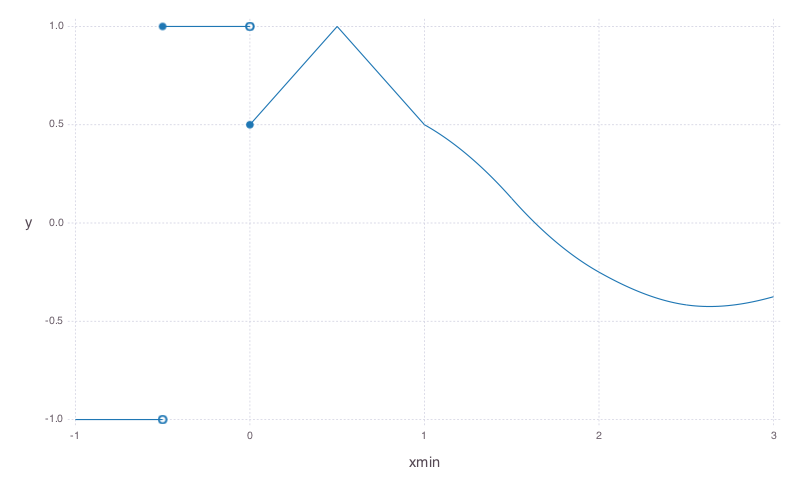
\includegraphics[width=\textwidth]{figures/piecewise-initial-function.png}
	%\caption{}
	\label{fig:not-allowed}
\end{figure}



\chapter{Introduction to Logic}
    \label{sec:introduction-logic}

    \section{First-Order Logic}
        \label{sec:first-order-logic}

        \textit{First-order logic} (\FOL) is a framework for studying rules of argument (\cite{hodges2001ClassicalLogic}) and will be used a means for the specification of properties of hybrid programs later on.

        We introduce first-order logic similiar to the definitions given in \cite{Platzer10HybridSystems} and \cite{Huth04LogicInCS}. More subtleties are adapted from \cite{hodges2001ClassicalLogic} and \cite{rautenberg10ConciseLogic}.
        % though with a different notation/nomenclature

        declarative sentences made of atomic, indecomposible sentences


        % it is predicate logic, not propositional
        propositional: no =, no quantifiers, no functions/predicates, only true/false constant symbols (= predicates of arity 0 = propositions)

        % TODO: truth values

        predicate logic

        First-order logic extends propositional logic,
        with quantifiers
        and variables
        and functions/predicates of arity $\geq 1$

        Propositional logic only deals with \textit{declarative sentences}, so-called \textit{propositions}, which can be declared as either true or false. and how these can be connected


        logical symbols (and, or, imply, not, forall, exists, equality???) (can partly be expressed by each other)
        parentheses
        extralogical symbols in signature
        logical variables
        all together: alphabet

        Functions take values as argument and give back a new value, which can be of any type. Function symbols stand for a function and are usually denoted by $f,g,h$.

        % FIXME: Zielraum in englisch
        difference between functions and predicates is Zielraum

        In contrast to functions, predicates return either true or false, depending on the values of their arguments.
        So depending on the context, a predicate symbol, usually written as $p,q,r$, is either true or false.

        The \textit{arity} of a function or predicate symbol is the number of arguments it demands.
        Functions can be of arity zero, i.e. without any argument.
        For clarity, we will treat these so-called \textit{constants} (or nullary functions) seperately and write their symbols as $a,b,c$.
        The arities are specified by the signature $\signature$.

        Variable symbols $x,y,z$ refer to objects

        Precisely define a set of symbols and their roles

        \subsection{Syntax}
            \label{sec:FOL-syntax}

            First-order logic inductively defines a syntax of well-formed \textit{logical formulae} over an alphabet containing different kinds of symbols.

            The syntax only defines rules which specify how the given symbols can be textually combined. At this stage, they have no specific meaning yet.

            The alphabet $\signature\cup\varsymbols$ comprises the \textit{signature} $\signature$ of the theory, which is a set of predicate, function and constant symbols, and the set of logical variable symbols $\varsymbols$.

            Terms are the expressions which denote feasible arguments for functions and predicates. always denotes an element of universe
            \begin{definition}[Terms]
                For a given \textit{signature} $\signature$ and set of variable symbols $\varsymbols$, the well-formed terms are either logical variables, constants or functions applied to terms:
                The set of all \textit{terms} $\terms$ is the smallest set with
                \begin{enumerate}
                    \item If $x\in\varsymbols$ then $x\in\terms$.
                    \item If $c\in\signature$ is a constant symbol, then $c\in\terms$.
                    \item If $f\in\signature$ is a function symbol of arity $n\geq 1$ and $\istrm{i}\in\terms$ for $i=\range{1}{n}$, then $f(\range{\istrm{1}}{\istrm{n}})\in\terms$.
                \end{enumerate}
                This definition can alternatively be written as grammar in Backus-Naur form
                \begin{equation}
                    \astrm,\istrm{i} \Coloneqq
                        x \mid
                        c \mid
                        f(\range{\istrm{1}}{\istrm{n}})
                \end{equation}
                where $x$ is ranging over the set of logical variables $\varsymbols$, $c$ over the nullary functions in $\signature$ and $f$ over the elements in $\signature$ with arity $n\geq 1$.
            \end{definition}

            Formulas are expressions which will admit truth values.
            \begin{definition}[First-Order Formulas]
                For given $\signature$ and $\varsymbols$, the well-formed formulas of a (first-order) logic are words formed by recursive combination of signature-symbols with logical operator symbols:
                The set of formulas $\FOLformulas$ is the smallest set with
                % TODO: term1=term2, or is this predicate?
                \begin{enumerate}
                    \item If $p\in\signature$ is a predicate symbol of arity $n\geq 0$ and $\istrm{i}\in\terms$ for $i=\range{1}{n}$ then $p(\range{\istrm{1}}{\istrm{n}})\in\FOLformulas$.
                    \item If $\asfml,\bsfml\in\FOLformulas$, then $\lnot\asfml,(\asfml\land\bsfml),(\asfml\lor\bsfml),(\asfml\limply\bsfml)\in\FOLformulas$.
                    \item If $\asfml\in\FOLformulas$ and $x\in\varsymbols$ then $(\lforall{x}{\asfml})\in\FOLformulas$ and  $(\lexists{x}{\asfml})\in\FOLformulas$.
                \end{enumerate}
                We may again write this as
                \begin{equation}
                    \asfml,\bsfml \Coloneqq
                        p(\range{\istrm{1}}{\istrm{n}}) \mid
                        \lnot\asfml \mid
                        \asfml\land\bsfml \mid
                        \asfml\lor\bsfml \mid
                        \asfml\limply\bsfml \mid
                        \lforall{x}{\asfml} \mid
                        \lexists{x}{\asfml}
                \end{equation}
                where $p\in\signature$ ranges over the predicate symbols (of arity $k\geq 1$), $\istrm{i}\in\terms$ over the terms and $x\in\varsymbols$ over the variable symbols.
            \end{definition}

        \subsection{Semantics}
            \label{sec:FOL-semantics}



            variable symbol = logical variable
            universe of objects, domain of discourse
            assign a value of universe to variable

            definition triplet universe,interpretation,assignment is called model

            The \textbf{semantics} of a first-order logic specify the meaning of each symbol occuring in terms and formulae with the goal to assign a \textbf{truth value} to a full formula.

            need concrete objects for symbols
            based on a valuation

            requires to fix a \textit{universe} of concrete values
            objects of consideration

            \begin{definition}[Universe]
                A non-empty set $\universe$ containing the concrete objects of discurse, is called \textit{universe}.
            \end{definition}

            \begin{definition}[Interpretation]
                An \textbf{interpretation} $\interpret$ assigns concrete elements to their corresponding symbols in a given signature $\signature$. It consists of
                \begin{enumerate}
                    \item For each constant symbol $c\in\signature$ a value $\interpret[c]\in\universe$.
                    % FIXME: proper function definitions, ie. : and arrow, \from\to
                    % TODO: reference to cartesian product
                    \item For each function symbol $f\in\signature$ of arity $k\geq 1$, $\interpret[f]\from\universe^k\to\universe$ is a function with $k$ arguments.
                    \item For each predicate symbol $p$ of arity $k\geq 1$, $\interpret[p]\subseteq\universe^n$ is a relation.
                \end{enumerate}

            \end{definition}

            % Interpretation associates $f$ with $\interpret{f}(\range{d_1}{d_n})\in\universe$ value of function at position $(\range{d_1}{d_n})\in\universe^k $

            The predicate $p$ is \textit{true} at position $(\range{d_1}{d_n})\in\universe^k$ under $\model$ if and only if $(\range{d_1}{d_n})\in\interpret[p]$.
            An alternative but equivalent formulation uses the characteristic function $\interpret[p]\from\universe^n\to\{\ltrue,\lfalse\}$, where $p$ is true at $(\range{d_1}{d_n})\in\universe^n$ if and only if $\interpret[p](\range{d_1}{d_n})=\ltrue$.

            % provide seperate characterisation, meaning of the connectives
            % truth tables
            % to define what is true and false
            % semantics is equivalent to proof theory


            % relationship
            % $\range{\asfml_1}{\asfml_n}\models\bsfml$
            % looking at truth values of atomic formulas in premises and conclusion, how manipulated by logical connectives, defined by a table for all possible cases
            % calculate truth value of formula from truth value of atomic propositions

            % classical logic \cite{reis2014cutelimination}
            % set of truth values true,false
            % every sentence always true or false
            % its sequent calculus is LK
            % valuation/model of a formula is an assignment of a truth value to each atomic proposition inside that formula


            assignment of logical variables
            Logical variables are only place holders and need, at some stage, refer to a concrete value. This interpretation is realized by an assignment.

            \begin{definition}[Assignment]
                An \textbf{assignment} is a map $\assignment\from\varsymbols\to\universe$ which assigns a value of the universe to each variable symbol $x\in\varsymbols$.
            \end{definition}

            \begin{definition}[Model]
                A model is the triplet $\model=(\universe,\interpret,\assignment)$ of a universe $\universe$, an interpretation $\interpret$ and an assignment $\assignment$.
            \end{definition}

            We write $\modif{\model}{x}{a}$ for the model which differs from the model $\model$ only in the assignment to the logical variable $x$, to which the value $a\in\universe$ is allocated.

            Given the information of a model, we can finally evaluate a formula, i.e. decide on its truth value.

            The valuation of terms and formulae is again defined inductively.
            \begin{definition}[Valuation of Terms]
                For $\terms$ the/a \textit{valuation} $\ivaluation{\IFOL}{\phi}$ is defined by
                \begin{enumerate}
                    \item $\ivaluation{\IFOL}{x} = \assignment(x)$ for each logical variable $x\in\varsymbols$
                    \item constant
                    \item $\ivaluation{\IFOL}{f(\range{\istrm{1}}{\istrm{n}})} = \interpret[f](\range{\ivaluation{\IFOL}{\istrm{1}}}{\ivaluation{\IFOL}{\istrm{n}}})$ for each function symbol $f\in\signature$ of arity $n\geq 1$.
                \end{enumerate}
            \end{definition}


            meaning of connective symbols, how they preserve a truth value
            defined as truth table
            translation into natural language?
            \begin{definition}[Valuation of First-Order Formulas]
                valuation of first-order formulas $\FOLformulas$
                in the interpretation $\interpret$
                under the assignment $\assignment$ is given by
                \begin{enumerate}
                    \item predicate $\ivaluation{\IFOL}{p(\range{\istrm{1}}{\istrm{n}})} = \interpret[p](\range{\ivaluation{\IFOL}{\istrm{1}}}{\ivaluation{\IFOL}{\istrm{n}}})$
                    \item The conjunction $\ivaluation{\IFOL}{\astrm\land\bstrm} = \ltrue$ iff $\ivaluation{\IFOL}{\astrm}=\ltrue$ and $\ivaluation{\IFOL}{\bstrm}=\ltrue$.
                    \item The disjunction $\ivaluation{\IFOL}{\astrm\lor\bstrm} = \ltrue$ iff $\ivaluation{\IFOL}{\astrm}=\ltrue$ or $\ivaluation{\IFOL}{\bstrm}=\ltrue$.
                    \item The negation $\ivaluation{\IFOL}{\lnot\astrm} = \ltrue$ iff $\ivaluation{\IFOL}{\astrm} \neq \ltrue$.
                    \item The implication $\ivaluation{\IFOL}{\astrm\limply\bstrm} = \ltrue$ iff $\ivaluation{\IFOL}{\astrm} \neq \ltrue$ or $\ivaluation{\IFOL}{\bstrm}=\ltrue$.
                    \item The universal quantifier $\ivaluation{\IFOL}{\lforall{x}{\astrm}} = \ltrue$ iff $\ivaluation{\imodif[algebra]{\IFOL}{x}{a}}{\astrm} = \ltrue$ for all $a\in\R$.
                    \item The existential quantifier $\ivaluation{\IFOL}{\lexists{x}{\astrm}} = \ltrue$ iff $\ivaluation{\imodif[algebra]{\IFOL}{x}{a}}{\astrm} = \ltrue$ for some $a\in\R$.
                \end{enumerate}

                The statement $\ivaluation{\IFOL}{\astrm}=\ltrue$ can also be written as $\imodels{\IFOL}{\astrm}$, the so-called \textit{satisfaction/satisfiability relation}.
                One says that $(\interpret,\assignment)$ \textit{satisfies} $\asfml$, that $(\interpret,\assignment)$ is a model for $\asfml$ or that $\asfml$ is \textit{true} in $\interpret$ under $\assignment$.

                A formula $\asfml$ is called \textit{valid} (or a \textit{tautology}) if $\imodels{\IFOL}{\asfml}$ for every model $\model$ (i.e. for all possible interpretations $\interpret$ and assignments $\assignment$). In this case, one writes shortly $\models\asfml$.
            \end{definition}
            formula is satisfieable, valid, or neither
            satisfieable if there is at least one model in which formula evaluates to true
            valid if always evaluates to true, in every model

        \subsection{Proof Theory}
        \label{sec:FOL-proof-theory}

            % FIXME: when to use vDash instead of models? because of \entails in semantics
            test $\models\vDash $ establish validity by proofs
            semantics: given interpretation,assignment -> compute its truth value, check satisfaction easy
            check validity difficult, need to check for all interpretations, assignments
            proofs shows validity, but not valid difficult, how to show that there is no proof?

            proof for establishing evidence of assertions, like $\lsequent{\Gamma}{\astrm}$ valid
            not useful for $\lsequent{\Gamma}{\astrm}$ not valid

            two characterisations need be equivalent, ie soundness and completeness

            valid formulas are of particular interest, hold under all circumstances, ie for all interpretations and assignments

            need to identify these, check validity

            if not valid, there is a counterexample, an interpretation and assignment for which not true, ie false

            can be hard to find such, but easy to check to be one

            want to easily show validity
            witness for not validity: counterexample
            witness for validity: (formal) proof

            formal proof is a derived formula, which is obviously valid
            form initial formula by valid rules

            can be difficult to find a proof
            but proof can easil be verified by validity of proof rules

            proof rules are derived from axioms or easy valid formulas

            different styles of formal logical argumentation

            deduction systems in which a proof can be represented

            proof of a sequent is a tree, initial sequent as root, axioms as leaves

            $w\models\Gamma$ means $w\models\asfml$ for all $\asfml\in\Gamma$
            definition
            logical consequence $\Gamma\models\bsfml$ if $w\models\bsfml$ for every model of $\Gamma$
            $w\models\Gamma\limply w\models\bsfml$ for all valuations w
            super charged symbol but context

            $T$ entails $\asfml$, all interpretations satisfying $T$ also satisfy $\asfml$
            $\asfml$ is valid, if every interpretation makes it true

            a sequent is deriveable/provable in proof calculus $C$, $T|-_C\asfml$ if there is a formal proof in the calculus for the sequent

            judgement of form
            \begin{equation}
                \lsequent{\range{\asfml_1}{\asfml_n}}{\bsfml}
            \end{equation}
            called sequent
            sets may be empty
            sequent is valid, if there is a proof

            proof calculus is sound if invalid sequents are not deriveable in C
            is complete if every valid sequent can be derived

            \subsubsection{Logical Axioms}
                \label{sec:FOL-axioms}

                theory of $\model$ is set of sentences satisfied by $\model$
                generally, theory is set of sentences
                model class of theory $T$: all interpretations which satisfy $T$ (all sentences given in T)
                if $K$ (interpretations) is model class of theory $T$, then $T$ is set of axioms for $K$ (\cite{hodges2001ClassicalLogic})

                zero-premise rule
                \begin{calculus}
                    \cinferenceRule[ax|]{}{
                        \linferenceRule[sequent]{}{\lsequent{\asfml}{\asfml}}
                    }{}
                \end{calculus}

            \subsubsection{Hilbert Calculus}
                \label{sec:hilbert-calculus}

                \cite{hodges2001ClassicalLogic}

                selected tautologies with role of axiom
                selection is rather arbitrary
                depending on signature

                inference rules

                modus ponens (MP)

                logical axiom scheme, all formulas of the form

                % TODO: axioms for Hilbert FOL
                \begin{calculus}
                    \cinferenceRule[L1|$\Lambda1$]{}{
                        \linferenceRule[impl]{(\asfml\limply(\bsfml\limply\csfml))}{(\asfml\limply\bsfml)\limply(\asfml\limply\csfml)}
                    }{}
                    \cinferenceRule[L2|$\Lambda2$]{}{
                        \linferenceRule[impl]{a}{a}
                    }{}
                    \cinferenceRule[L3|$\Lambda3$]{}{
                        \linferenceRule[impl]{a}{a}
                    }{}
                    \cinferenceRule[L4|$\Lambda4$]{}{
                        \linferenceRule[impl]{a}{a}
                    }{}

                \end{calculus}

                are all tautologies

                Hilbert Style deduction system/calculi
                every line of a proof is unconditional tautology or theorem

                small number of inference rules
                relying more on axioms

                reach a conclusion by applying deduction rules to axioms

                useful when one wants to add further axioms to first-order base

                judgement is any formula of given (first-order) logic
                theorems: formulae appearing in concluding judgement of a valid proof $\lsequent{}{\bsfml}$

                define class of axioms, ie the set of all formulas which have any of the forms ...

                formal proof is a derivation of the formula (conclusion) from axioms and premises by applying in each step modus ponens or quantifier-generalization

                $\bsfml$ deriveable in C from premises, if exists a derivation with conclusion $\bsfml$

                lemma to be used in another proof


            % TODO: natural deduction calculus
            \subsubsection{Natural Deduction}
                \label{sec:natural-deduction}

                The \textit{natural deduction} is a calculus in the so-called Gentzen style,
                which relies on only a few axioms but an exhaustive collection of inference rules operating on sequents.

                By applying these rules one infers formulas from formulas and finally deduces a conclusion from the given set of promises.

                % ??? oder mehrere premises (sequents) oben one unten
                Every line of a proof is a conditional tautology, with zero or more conditions on the left side of the sequent and exactly one asserted proposition on the right hand side.

                premises: set of formulas $\range{\asfml_1}{\asfml_n}$
                conclusion $\bsfml$ single formula

                umforme premises with rules into conclusion
                this intention, written as
                from premisses conclude conclusion $\bsfml$


                in contrast to relationship $\range{\asfml_1}{\asfml_n}\models\bsfml$, see semantics

                Finding a proof can be difficult, because it might not be obvious which proof rules need to be applied and in what order.

                theorems: formulae appearing in concluding judgement of a valid proof $\lsequent{}{\bsfml}$

                % TODO: add ref to soundness
                rules well chosen, see soundness

            \subsubsection{Sequent Calculus}
                \label{sec:sequent-calculus}

                Gentzen style
                zero or more asserted propositions

                can be regarded as Hilbert-style calculus for deriving finite sequences instead of formulas \cite{hodges2001ClassicalLogic}

                sequent is a standard form for logical formulas
                antecedent $\Gamma$ assumed to be true
                succedent $\Delta$ one of these to be shown
                both finite sets of formulas
                $\lsequent{\Gamma}{\Delta}$, which means
                \begin{equation}
                    \landfold_{\asfml\in\Gamma}\asfml \limply \lorfold_{\bsfml\in\Delta}\bsfml
                \end{equation}

                comma in antecedent like conjunction, in succedent like disjunction
                rules decompose propositional structure of a formula leading to simpler ones

                empty sequent, both side empty, defined to be false
            % or sequent calculus
            % Gentzen, Hilbert
            % TODO: Bruch schreibweise, not iff, only if

            % TODO: free variables
            free variable: needs an object assigned in order to determine a truth valua for formula
            bound variable: no assignment needed
            sentence is formula without free variables, has a determined truth value
            quantifiers bind occurences of variable in formula
            sentence: formula without free formula



            \subsubsection{Proof Rules}
                \label{sec:FOL-proof-rules}


                two groups: logical (operate on formula and sub-formulas) and structural (such as contraction=copy, weakening=erase, cut)

                %prop logic rules + rules for = and quantifiers

                sequent below horizontal line: conclusion
                sequents above horizontal line: premises

                \paragraph{Universal Quantification Rules}
                    % TODO: forall e <-> forall i
                    eliminates $\forall$
                    $\lforall{x}{\asfml}$ is true if we can replace quantified variable by any term (side condition, $\astrm$ needs be free for x in $\asfml$) and this remains true

                    \begin{calculus}
                        \cinferenceRule[FOLforall|$\forall$]{}{
                            \linferenceRule[sequent]{
                                \subst[\asfml]{x}{\astrm}
                            }{
                                \lforall{x}{\asfml}
                            }
                        }{}
                    \end{calculus}

                    soundness self-evident, since true for all, also for more concrete instance

                    \begin{example}
                        necessity for free

                    \end{example}

                \paragraph{Existential Quantification Rules}
                    % TODO: exists e <-> exists i
                    exists introduction

                    \begin{calculus}
                        \cinferenceRule[FOLexists|$\exists$]{exists generalization rule}{
                            \linferenceRule[sequent]{
                                \lexists{x}{\asfml}
                            }{
                                \subst[\asfml]{x}{\astrm}
                            }
                        }{}
                    \end{calculus}

                    $\astrm$ free for $x$ in $\asfml$
                    can deduce $\lexists{x}{\asfml}$ if we know that true for a concrete instance, witness

            \subsubsection{Ground Proving and Free Variable Proving}
                \label{sec:ground-proving-free-variable-proving}



        \subsection{First-Order Logic of Real Arithmetic}
            \label{sec:FOL-R}

            first-order logic of real arithmetic (\FOLR)
            formula of real arithmetic
            is first-order formula
            function/predicate symbols $ = {+,-,\cdot,/,=,<,\leq,>,\geq}$
            constant symbols $\Sigma$
            logical Variables $V$

        \subsection{Decideability}
            \label{sec:decideability}

            (\cite{hodges2001ClassicalLogic})
            language (e.g. FOL) decideable if there is an algorithm which returns for any finite sequent if it is valid or not

        \subsection{Correctness}
            \label{sec:correctness}

            $\bsfml$ deriveable from premises, then sequent is valid

        \subsection{Completeness}
            \label{sec:completeness}

            given a valid sequent, then conclusion is deriveable from premises

        % \subsubsection{Substitution}
        % \label{sec:substitution}
        %
        % variables are place holders
        % means of replacing with concrete information


\chapter{Hybrid Programs with DDEs}\label{hybrid-programs-with-ddes}

We extent hybrid programs (\HPs) and formulae of classical \dL with syntax, semantics, axiomatization and proof rules which allow to deal with Delay Differential Equations.
%Is a super set, \dL is a fragment
Call obtained \dHPs and \ddL.

Similiar to first-order logic and essentially as an extension of dL we define delay differential logic

\cite{Platzer12Complete,Platzer15Uniform}

\section{Example}
    \label{example-hp-cars}
    To motivate the need of being able to treat Delayed Differential Equations in hybrid programs, we present some examples.

    \subsection{Leading and Following Car}

    \subsection{Network Induced Delay in Control Loops}

\section{Syntax}
    \label{sec:syntax}

    The syntax of \ddL terms, formulae as well as of \dHPs is defined inductively by a grammar in Backus-Naur-form (BNF).

    Let $\allvars$ be the set of \emph{all variables} and $\diffvars\defeq\{\D{x} \with x\in\allvars\}$ the corresponding set of \emph{differential symbols}.
    Let $\constants$ be the set of \emph{all constants}. We denote $\delayvars\defeq\{\xtau[c] \with x\in\allvars, c\in\constants\}$ the set of \emph{delayed variables} and $\diffvars\times\constants\defeq\{\Dxtau[c] \with \D{x}\in\diffvars, c\in\constants\}$ the set of \emph{delayed differentials}.

    We will usually denote variables by $x,y,z\in\allvars$ and their differential symbols by $\D{x},\D{y},\D{z}\in\diffvars$.

    Function symbols $f,g,h$, constant symbols $a,b,c$ and predicate symbols $p,q,r$ are as in first-order logic (cf. Section \ref{sec:first-order-logic}).

    % FIXME: what are program constants?
    %program constants $ $, may be in $\rationals$

    \begin{definition}[Terms]\label{def:syntax-terms}
        \emph{Terms} are defined by the following grammar, extending \dL with symbols for \emph{delayed variables} and \emph{differentials}:
        \begin{equation*}
            \astrm,\bstrm \Coloneqq
                \xtau[s] \mid
                \Dxtau[s] \mid
                % TODO: maybe dont need x[c], only with s and use t(s) with specified s, as in DDE and extra x[0]=x
                \xtau[b] \mid
                \Dxtau[b] \mid
                c \mid
                f(\range{\istrm{1}}{\istrm{k}}) \mid
                \astrm + \bstrm \mid
                \astrm \cdot \bstrm \mid
                % FIXME: is term' allowed? diff inv is only a FOLR formula? even for dL valid?
                \D{(\astrm)}
        \end{equation*}
        % TODO: line breaks and explination text in syntax
        % \begin{align}
        %     \astrm\Coloneqq{}&\\
        %     &\mid \astrm+\bstrm\hfill\text{test}
        % \end{align}
        where $x\in\allvars,\D{x}\in\diffvars$ and $f$ is a function symbol of arity $k$.
        The symbol $c\in\constants$ defines a rational number constant and $b\in\Q_{\leq 0}$.
        All terms implicitely depend on a time parameter $s\in\R_{\leq 0}$, written as $\astrm(s)$. When $s=0$ we abbreviate the notation to $\astrm$.
        The variable symbol $x$ and the differential symbol $\D{x}$ are the only ones which allow explicitely mentioning this parameter. They are spelled slightly differently using square brackets as $\xtau[s]$ and $\Dxtau[s]$, respectively. Note that $s\notin\allvars\cup\diffvars\cup\constants$. It is a special variable.
        In particular, for $\xtau[0]$ we write $x$ and $\D{x}$ for $\Dxtau[0]$.

        Writing $\astrm(-\tau)$ means that all occurences of $s$ in $\astrm$ have been replaced with $-\tau$.
        parameter is inherited

        % TODO: subtraction and division in terms

        %The symbol $x$ is only allowed in the right hand side of a DDE and in evolution domain constraints, not in other formulas. The latter may only contain $\xtau$.
    \end{definition}

    \begin{example}
        Let us consider the \ddL term
        \begin{equation}
            \astrm(s) = \underbrace{\xtau[s]}_{\text{var}} + \underbrace{\xtau}_{\text{const}}.
        \end{equation}
        Setting $s=-1$ gives the term
        \begin{equation}
            \astrm(-1) = \xtau[-1] + \xtau.
        \end{equation}
    \end{example}

    The grammar defining \emph{delayed hybrid programs} is the same as for classical \HPs (cf. \cite{Platzer15Uniform}) and is shown here for completeness.

    \begin{definition}[(Delay) Hybrid Programs]\label{def:syntax-HP}
        \emph{(Delay) Hybrid programs} (\dHPs) are defined by
        % TODO: first-order logic of real arithmetic formulas include \xtau?
        \begin{equation*}
            \asprg, \bsprg \Coloneqq
                a \mid
                % FIXME: do I need theta(0), or can I later just say, s not free in theta ?
                \hupdate{\humod{x}{\astrm(0)}} \mid
                \Dupdate{\Dumod{\D{x}}{\astrm(0)}} \mid
                \htest{\asfmlfolR} \mid
                \hchoice{\asprg}{\bsprg} \mid
                % TODO: replace ; in HPs
                \asprg;\bsprg \mid
                \hrepeat{\asprg} \mid
                \hevolvein{\D{x}=\astrm(-\tau)}{\ivr}
        \end{equation*}
        % TODO: ddes with mult const delay
        % TODO: program constant
        where $\asprg, \bsprg$ denote \dHPs, with a variable $x$, a term $\astrm$ (possibly containing $x$ or $\xtau$) and $\ausprg$ a program constant.
        The formula $\asfmlfolR$ is of first-order logic of real arithmetic \FOLR$(\allvars)$, containing only normal variable symbols $\allvars$.
        Note: $s\notin\asprg$.
        Syntax only allows autonomous DDEs.
    \end{definition}

    

    The difference between classical \HPs (in the sense of ...) and \dHPs is not syntactically, but only given by their semantics.

    refer to Section \ref{sec:dynamic-semantics} for meaning of the following, different meaning for formulae

    assignment, discretely at an instant of time
    test of formula in current state
    nondeterministic choice
    sequential composition
    nondeterministic repetition
    delay differential equation with restricted evolution, due to domain constraint $\bsfml$, follow arbitrary amount of time
    DDE with delay tau, term has only $x$ and $\D{x}$ with constant nor var $s$
    ODE still possible


    \begin{definition}[\ddL Formulas]\label{def:syntax-formula}
        The \emph{formulae} of \emph{delay differential dynamic logic} (\ddL) are defined by
        \begin{align*}
            \asfml,\bsfml \Coloneqq{}& % fixes missing space
                % TODO: better abbreviated notation for \holdssince, make forall only appear in semantics rhs
                \astrm\geq\bstrm \mid
                p(\range{\istrm{1}}{\istrm{k}}) \mid
                \contextapp{C}{\asfml} \mid
                \lnot\asfml \mid
                \asfml\land\bsfml \mid\\
                &\holdssince{T}{\asfml(s)} \mid
                \lforall{x}{\asfml} \mid
                \lexists{x}{\asfml} \mid
                \dbox{\asprg}{\asfml} \mid
                \ddiamond{\asprg}{\asfml}
        \end{align*}
        with \ddL terms $\astrm,\bstrm,\range{\istrm{1}}{\istrm{k}}$,
        a predicate symbol $p$, a quantifier symbol $C$, a variable $x$, and a \dHP $\asprg$.
        
        % TODO: need = in formulas ?
        Other operators
        $\sim$ for $=,<,\leq,>,\geq$, such as $\lor,\limply,\lbisubjunct$ can be derived from $\land,\lnot$ and are hence not explicitely mentioned in the grammar.

        modal formula $\dbox{\asprg}{\asfml}$ : $\asfml$ holds in the state after all runs of $\asprg$, dual: there is a run
        % TODO: what is a quantifier symbol? (-> US paper)
        quantifier symbols $C$, with formula as argument are higher order predicate symbols and bind the variables of $\asfml$

        The quantifiers $\forall$ and $\exists$ quantify over $\statespace$.

        The symbol $T$ is a symbolic constant related to the history duration induced by the occurence of a delay-differnetial equation. Its value is set by proof rules.
    \end{definition}

    % TODO: FOLR is subset of ddL formulae
    \FOLR formulae are a subset of \ddL.

    When terms do not depend on quantified parameter, can omit writing down forall in formula

\section{Dynamic Semantics}
    \label{sec:dynamic-semantics}

    % TODO: state space pw diffable
    Following the remark to the solution of a DDE (cf. Section \ref{sec:definition-of-solution}), we define the \emph{state space} in \ddL to $\statespace$, the set of piecewise continuous functions on $\delayinterval$, as defined in Definition~\ref{def:piecewise-continuous}.

    This means that a variable remembers a limited part of its evolution history, what demands hence an implicit notion of a underlying time.

    We denote by $\states$ the \emph{set of states}. A \emph{state} $\asstate\in\states$ is a mapping
    \begin{equation}
        \asstate \from \allvars\cup\diffvars \to \statespace
    \end{equation}
    which assigns a \emph{history} (function) to each variable and differential symbol.

    By $\modif{\asstate}{x}{r}$ we denote the state which is equal to state $\asstate$, except for the value of the variable $x$ which is set to $r\in\statespace$.

    % FIXME: modification of x in state and general specification of pw function associated to x
    %at the time $t=0$. The value of $x$ for the time before does not change.

    % TODO: Abgrenzung zu Trace Semantics
    % The temporal character of delay differential equations (they depend on their own temporal evolution with limited horizon) suggests the introduction of trace semantics.
    %
    % However, we go the way of introducing transition semantics with an augmented state space.

    \begin{definition}[Semantics of terms]\label{def:sematic-terms}
        The \emph{semantics} of a term $\astrm$ in the state $\asstate\in\states$ (at time instant $t$) is a value in $\R$ and defined inductively as follows:
        \begin{enumerate}
            \item $\ivaluation{\IddL}{\xtau[s]} = \asstate(x)(s)$ for a variable $x\in\allvars$
            % FIXME: need Cpw for derivatives or only \R?
            \item $\ivaluation{\IddL}{\Dxtau[s]} = \asstate(\D{x})(s)$ for a differential symbol $\D{x}\in\diffvars$
            \item $\ivaluation{\IddL}{\xtau[b]} = \asstate(x)(b)$ for a variable $x\in\allvars$ and a constant $b\in\constants$ with $\interpret[b]\in\Q_{\leq 0}$
            \item $\ivaluation{\IddL}{\Dxtau[b]} = \asstate(\D{x})(b)$ for a differential symbol $\D{x}\in\diffvars$ and a constant $b\in\constants$ with $\interpret[b]\in\Q_{\leq 0}$
            \item $\ivaluation{\IddL}{c} = \interpret[c]$ for a constant $c\in\constants$
            \item $\ivaluation{\IddL}{f(\range{\istrm{1}}{\istrm{k}})} = \interpret[f](\range{\ivaluation{\IddL}{\istrm{1}}}{\ivaluation{\IddL}{\istrm{k}}})$ for a function symbol $f$
            \item $\ivaluation{\IddL}{\astrm+\bstrm} = \ivaluation{\IddL}{\astrm} + \ivaluation{\IddL}{\bstrm}$
            \item $\ivaluation{\IddL}{\astrm\cdot\bstrm} = \ivaluation{\IddL}{\astrm} \cdot \ivaluation{\IddL}{\bstrm}$
            % FIXME: derivation of terms with x'?
            \item $\ivaluation{\IddL}{\D{(\astrm)}} = \displaystyle\sum_{c\in\constants\cup\set{s}} \asstate(\D{x})(\interpret[c])\frac{\partial\ivaluation{\IddL}{\astrm}}{\partial \xtau[c]}$
        \end{enumerate}
        %where $s\in [-T,0]$.
        The  syntactic (total) derivation, defined in \ref{def:derivation}, gives new term
    \end{definition}
        % TODO: mention 'interpretation' for semantics.
        % FIXME: interpretation of $f$ is a smooth function


    % TODO: total derivative operator for terms
    \begin{definition}[Derivation]\label{def:derivation}
        common derivation rules
        $\D{(\xtau[b])}=\Dxtau[b]$ need in premise $\D{x}$ on $[t+b,t]$
    \end{definition}

    % The semantic of the new symbol $\xtau$ depends on the context in which the term occures:
    % \begin{enumerate}
    %     \item in a hybrid program: $\imodel{\IddL}{\xtau} = \imodel{\IddL}{x(t-\tau)} = \nu(x)(-\tau)\in\R$
    %     \item in a formula $\xtau\in\statespace$: \begin{equation}
    %         % FIXME: rechte seite noch nicht korrekt
    %         \imodel[]{}{\phi(\xtau)} =
    %         \{\nu\in\states : \lforall{t\in[-\tau,0]}{\phi(\nu(x)(t))} \}
    %     \end{equation}
    %     with uniform substitution: $\sigma=\{\xtau\rightarrow\theta_0\}$
    % \end{enumerate}

    The meaning of a differential symbol: defined by state, 
    The time derivative of a variable may not be defined in isolated state, because it might have a discontinuity here and we cannot use its history (provided by the state) to define derivative.
    However, we can define a state local semantics for a differential $\D{(\astrm)}$.

    Like for ODE case, only use last value given in state. Since in $t=0$ could be incontinuity 

    chain rule for $\astrm(s)$
    $\asfml$ only mentions finitely many variables, finite sum
    $\ivaluation{\IddL}{\D{(\astrm)}}(s)$ is smooth as composition of smooth functions, derivatives exist

    Along a solution of a DDE $\varphi:[0,r]\rightarrow\states$ (continous differentiable), the differential symbols are interpreted as time derivatives, $r>0$ at any $\zeta\in[0,r]$, meaning of symbol is rate of change of value of $x$ over time
    \begin{equation}
        % TODO: replace \DD with Andres command
        \imodel{\IddL}{\D{x}}\varphi(\zeta)
            = \varphi(\zeta)(\D{x})(0)
            \defeq \DD{\varphi(t)(x)(0)}{t}(\zeta)
            = \DD{\imodel{\IddL}{x}\varphi(t)}{t}(\zeta)
    \end{equation}
    if $r=0$
    and what if there is no ODE/DDE given: in a given state should also be real value
    
    in initial state an arbitray value is allowed, will then sync with equation to fullfil $\varphi(\zeta)(\D{x})=\imodel{\IddL}{f(x)}\varphi(r)$
    initial value $\asstate(\D{x})$ may not be compatible with derivative
    final values coincide

    In the precondition, no values are associated to the differential symbols. In general, the initial function is only piecewise continuous.
    Since for later time instances, the values of the differential symbols derive from the DDE, they become (locally) smooth function.

    \begin{definition}[Semantics of \ddL formulae]\label{def:semantic-formulae}
        The semantics of a \ddL formula $\asfml$ is the subset of all states $\imodel{\IddL}{\asfml}\subseteq\states$ in which $\asfml$ is true. This set is given inductively by
        % TODO: mention interpretation I
        % FIXME: what is difference between \imodel and \ivaluation?
        % terms: ivaluation, formula: imodel, programms: ireachability
        \begin{enumerate}
            % TODO: replace : in set by \with
            % FIXME: change ':' in sets to '|'
            % FIXME: use notation forall ... : ...
            % FIXME: *version for lforall without parentheses
            %\item $\imodel{\IddL}{\holdssince{T}{\astrm\geq\bstrm}} = \left\{\asstate\in\states \with \holdssince{T}{\ivaluation{\IddL}{\astrm(s)}\geq\ivaluation{\IddL}{\bstrm(s)}}\right\}$
            %\item $\imodel{\IddL}{\holdssince{T}{p(\range{\istrm{1}}{\istrm{k}})}} = \left\{\asstate\in\states \with \holdssince{T}{\left(\range{\imodel{\IddL}{\istrm{1}(s)}}{\imodel{\IddL}{\istrm{k}(s)}}\right)\in\interpret[p]}\right\}$
            \item $\imodel{\IddL}{\astrm(s)\geq\bstrm(s)} = \left\{\asstate\in\states \with \ivaluation{\IddL}{\astrm(s)}\geq\ivaluation{\IddL}{\bstrm(s)}\right\}$
            \item $\imodel{\IddL}{p(\range{\istrm{1}(s)}{\istrm{k}(s)})} = \left\{\asstate\in\states \with \left(\range{\ivaluation{\IddL}{\istrm{1}(s)}}{\ivaluation{\IddL}{\istrm{k}(s)}}\right)\in\interpret[p]\right\}$
            \item $\imodel{\IddL}{\contextapp{C}{\asfml}} = \interpret[C]\left(\imodel{\IddL}{\asfml}\right)$ for a quantifier symbol $C$
            \item $\imodel{\IddL}{\lnot\asfml} = \scomplement{\left(\imodel{\IddL}{\asfml}\right)} = \states\setminus\imodel{\IddL}{\asfml}$
            \item $\imodel{\IddL}{\asfml\land\bsfml} = \imodel{\IddL}{\asfml}\cap\imodel{\IddL}{\bsfml}$
            \item $\imodel{\IddL}{\holdssince{T}{\asfml(s)}} = \left\{\asstate\in\states \with \holdssince{T}{\asstate\in\imodel{\IddL}{\asfml(s)}} \right\}$
            \item $\imodel{\IddL}{\lforall{x}{\asfml}} = \{\asstate\in\states \with \modif{\asstate}{x}{y}\in\imodel{\IddL}{\asfml} \text{ for all } y\in\statespace \}$
            \item $\imodel{\IddL}{\lexists{x}{\asfml}} = \{\asstate\in\states \with \modif{\asstate}{x}{y}\in\imodel{\IddL}{\asfml} \text{ for some } y\in\statespace \}$
            \item $\imodel{\IddL}{\dbox{\asprg}{\asfml}} = \{\asstate\in\states \with \bsstate\in\imodel{\IddL}{\asfml} \text{ for all $\bsstate$ such that} (\asstate,\bsstate)\in\ireachability{\IddL}{\asprg}\}$, i.e. $\{\asstate\in\states \with \lforall{\bsstate\in\states}{((\asstate,\bsstate)\in\ireachability{\IddL}{\asprg} \limply \bsstate\in\imodel{\IddL}{\asfml})}\}$
            \item $\imodel{\IddL}{\ddiamond{\asprg}{\asfml}} = \{\asstate\in\states \with \bsstate\in\imodel{\IddL}{\asfml} \text{ for some $\bsstate$ such that} (\asstate,\bsstate)\in\ireachability{\IddL}{\asprg}\}$, i.e. $\{\asstate\in\states \with \lexists{\bsstate\in\states}{((\asstate,\bsstate)\in\ireachability{\IddL}{\asprg} \land \bsstate\in\imodel{\IddL}{\asfml})}\}$
        \end{enumerate}
        The fact that formula $\asfml$ is true in state $\asstate$ under the interpretation $\interpret$, i.e. $\asstate\in\imodel{\IddL}{\asfml}$ can also be written as $\imodels{\IddL}{\asfml}$.
        A formula $\asfml$ is called valid, written as $\models\asfml$, if and only if $\asfml$ is true in all states under all interpretations.
    \end{definition}

    interpretation of predicate symbol, arity n: relation $I(p)\subseteq\R^n$
    interpretation of a quantifier symbol: functional $I(C):M\subseteq\states\to P(\states)$ maps subsets of states to subsets of states

    Atomic formulas (type 1 and 2) need to be combined with the quantification over s (6) in order to make sense. See Section \ref{sec:well-definedness}.

    With the semantics of terms if follows for the meaning of $\dbox{\asprg}{\phi}$, that $\phi$ must only hold up to time $\tau$ before leaving the \HP $\asprg$. It is possible, that $\phi$ was not verified before, while \emph{executing} the \HP.

    However when we apply the Rule of steps, we get the validity of $\phi$ for the entire trace.

    % TODO: is it better to only have xtau and not choice? What if both mentioned?
    in formulae (such as safety condition or evolution constraint), we have two possibilities: only value at current time instant ($x$) or for entire last $\tau$ time $\xtau$

    $\dbox{}{}$ and $\ddiamond{}{}$ only refer to last state and not intermediate states, as \dTL does.

    % TODO: Move to static semantics
    If no dependance on $s$ in terms, $\holdssince{T}{}$ can be dropped in formula.

    \begin{example}
        Consider the two well-formed \ddL formulae:
        \begin{align*}
            &\holdssince{T}{x+\xtau[s]\geq 0}\\
            &\holdssince{T}{x+\xtau\geq 0} 
        \end{align*}
        The quantification over $s$ in the second formula can be dropped.
    \end{example}

    % TODO: do we accept that or restrict formula after modality to not having $s$ free? then, since s\notin\asprg commutes also for diamond
    \begin{lemma}
        The box modality and the quantification over $s$ commute
        \begin{equation*}
            \imodel{\IddL}{\holdssince{T}{\dbox{\asprg}{\asfml(s)}}} = \imodel{\IddL}{\dbox{\asprg}{(\holdssince{T}{\asfml(s)})}}
        \end{equation*}
    \end{lemma}
    \begin{proof}
        Since $\lforall{x}{p\limply q(x)}\equiv p\limply\lforall{x}{q(x)}$, it holds
        \begin{multline*}
            % FIXME: use \set instead of {}
            \imodel{\IddL}{\holdssince{T}{\dbox{\asprg}{\asfml(s)}}}\\
            = \set{\asstate\in\states \with \holdssince{T}{\lforall{\bsstate\in\states}{(\asstate,\bsstate)\in\ireachability{\IddL}{\asprg} \limply \bsstate\in\imodel{\IddL}{\asfml(s)}}}}\\
            = \set{\asstate\in\states \with \lforall{\bsstate\in\states}{\holdssince{T}{(\asstate,\bsstate)\in\ireachability{\IddL}{\asprg} \limply \bsstate\in\imodel{\IddL}{\asfml(s)}}}}\\
            = \set{\asstate\in\states \with \lforall{\bsstate\in\states}{(\asstate,\bsstate)\in\ireachability{\IddL}{\asprg} \limply \holdssince{T}{\bsstate\in\imodel{\IddL}{\asfml(s)}}}}\\
            = \set{\asstate\in\states \with \lforall{\bsstate\in\states}{(\asstate,\bsstate)\in\ireachability{\IddL}{\asprg} \limply \bsstate\in\imodel{\IddL}{\holdssince{T}{\asfml(s)}}}}\\
            = \imodel{\IddL}{\dbox{\asprg}{(\holdssince{T}{\asfml(s)})}}
        \end{multline*}
    \end{proof}
    
    However, the diamond modality does not commute with the s-quantification.
    % TODO: is this a problem? or okay?
    \begin{equation}
        \imodel{\IddL}{\holdssince{T}{\ddiamond{\asprg}{\asfml(s)}}} \neq \imodel{\IddL}{\ddiamond{\asprg}{(\holdssince{T}{\asfml(s)})}}
    \end{equation}

    Since, with respect to \dL, the state space has been replaced, we need to redefine the semantics.
    
    \begin{definition}[Transition semantics of \HPs]\label{def:semantic-HP}
        The interpretation of a \HP is given by a binary \emph{reachability relation} $\ireachability{\IddL}{\asprg}\subseteq\states\times\states$ between states:
        \begin{enumerate}
            \item $\ireachability{\IddL}{a} = \interpret[a]$ for a program constant $a$
            \item $\ireachability{\IddL}{\hupdate{\humod{x}{\astrm}}} =
                \left\{(\asstate,\bsstate)\with \bsstate = \asstate \text{ except }
                \bsstate(x) = \left(s\mapsto\begin{cases}
                    \ivaluation{\IddL}{\theta(s)} & s=0\\
                    \asstate(s) & s\in[-T,0)
                \end{cases}\right)\right\}$
            \item $\ireachability{\IddL}{\Dupdate{\Dumod{\D{x}}{\astrm}}} =
                \left\{(\asstate,\bsstate)\with \bsstate = \asstate \text{ except }
                \bsstate(\D{x}) = \left(s\mapsto\begin{cases}
                    \ivaluation{\IddL}{\theta(s)} & s=0\\
                    \asstate(s) & s\in[-T,0)
                \end{cases}\right)\right\}$
            \item $\ireachability{\IddL}{\htest{\asfmlfolR}} = \left\{(\asstate,\asstate) \with \asstate\in\imodel{\IddL}{\asfmlfolR} \right\}$
            \item $\ireachability{\IddL}{\hchoice{\asprg}{\bsprg}} = \hchoice{\ireachability{\IddL}{\asprg}}{\ireachability{\IddL}{\bsprg}}$
            \item $\ireachability{\IddL}{\asprg;\bsprg} = \left\{ (\asstate,\bsstate) \with (\asstate,\csstate)\in\ireachability{\IddL}{\asprg}, (\csstate,\bsstate)\in\ireachability{\IddL}{\bsprg} \right\}$
            \item $\ireachability{\IddL}{\hrepeat{\asprg}} %= \hrepeat{(\ireachability{\IddL}{\asprg})}
                = \displaystyle\cupfold_{n\in\N}\ireachability{\IddL}{\asprg^n}$ with $\asprg^{n+1}\equiv (\asprg^n;\asprg)$ and $\asprg^0\equiv \htest{\ltrue}$
            \item $\ireachability{\IddL}{\hevolvein{\D{x}=\astrm(-\tau)}{\ivr}} = \{
                (\asstate,\bsstate) \with
                \lforall{\zeta\in[0,r]}{\trajectory(\zeta)\in\imodel{\IddL}{\hevolve{\D{x}=\astrm(-\tau)}\land\ivr}}$
                and $\asstate=\trajectory(0)$ on $\scomplement{\{\D{x}\}}$ and $\bsstate=\trajectory(r)\}$, i.e. there exists a $r\geq 0$ and a trajectory $\trajectory\from [0,r]\to\states$, which fulfills $\trajectory(\zeta)(\D{x})(s) \defeq \DD{\trajectory(t)(x)(s)}{t}(\zeta) \stackrel{!}{=} \ivaluation{\iconcat[state=\trajectory(\zeta)]{\IddL}}{\theta}(s)$ (?) for all $s\in(-\min\{\zeta,T\},0]$
        \end{enumerate}
    \end{definition}

    $\trajectory$ solves the DDE and satisfies $\ivr$ in each time instant/state

    The formula $\hevolve{\D{x}=\astrm(-\tau)}\land\ivr$ has dropped the $\holdssince{T}{}$, alloccurences of $x$ and $\D{x}$ of form with constant

    if $r=0$: 

    For the \emph{discrete assignment}, we only allow the values at the current time instant to be changed. A functional assignment would essentially allow to rewrite history, which is not permitted.

    This assignment is the actual reason why we need to consider piecewise continuous evolutions.

    

    %TODO: super dense time: multiple assignments, only consider last assignment

    Using the extended syntax, we can write down both a delay differential equation and an ordinary differential equation in the form $\D{x}=\theta$, where $\theta=f(x,\xtau)$ with a polynomial $f$.

    Along a DDE/ODE, values of differential symbols coincide with time derivative of value of corresponding variable
    Remember that a $\xtau$ mentioned in $\theta$ here means $\varphi(t)(x)(-\tau)$.
    And so needs $\ivr$ always just hold at the current time instant (and not over the entire interval $[-\tau,0]$). The same case for $\ptest\psi$.

    \begin{definition}\label{def:termvars}
        define
        \begin{equation*}
            % FIXME: another symbol for defeq
            % TODO: what if x'[] in term ?
            \constants[\astrm] \defeq \set{c\in\constants \with \mexists{\xtau[c]\in\delayvars}\holds\xtau[c]\in\astrm}
        \end{equation*}
        does not contain $s$, since not in $\constants$
        Since a term only depends on a finite number of atomic terms for a fixed s
        can see valuation as a mapping from values of these symbols to reals
        instead of from functional space
        $\augtrajectory[s]{\astrm}\from\compactum{0}{r}\to\R^{\abs{\delayvars[\astrm]}}$
        \begin{equation*}
            \augtrajectory[s]{\astrm}(t) \defeq \colvec{\trajectory(t)(x)(c_1)\\ \vdots\\ \trajectory(t)(x)(c_n)}
        \end{equation*}
    \end{definition}
    % TODO: alternatively, could maybe have \trajectory Fréchet-diffable

    for formula not possible, since it depends possibly on infinitely many different values for s

    \begin{lemma}[Differential Lemma]\label{lm:differential-lemma}
        lecture notes L10.20
        needed for DI proof
        no changes, except for rewriting $\varphi(t)(x)\rightarrow\varphi(t)(x)(0)$
        [eta] is diffable with d/dt[eta]=[(eta)']
    \end{lemma}
    \begin{proof}
        % TODO: what if x'[] in term ?
        % TODO: in init cond: x and x' need to match, ie d/ds x[s] = x'[s], same subdivision, specification of x' in init cond only needed when referenced to it later
        % FIXME: oBdA: t_0=0
        Let $\trajectory\from\compactum{0}{r}$
        % FIXME: new statespace C^1_pw
        and $\subdivision{-T=t_0}{t_m=0}$ the subdivision of $\trajectory(0)(x)\in\statespace$.
        We show that value of a term is piecewise differentiable with subdivision $\mathcal{Z}$.

        Let $s\in\compactum{-T}{0}$ beliebig aber fest. Means $s$ is in the following a constant, like $c$.
        Let $\mathcal{Z}_\bstrm^s=\subdivision{\hat{t}_0}{\hat{t}_k}$ be the subdivision of the term $\bstrm$
        is subdivision of $\compactum{0}{r}$
        % FIXME: what when r>T ? Z={0,r}
        \begin{equation*}
            \mathcal{Z}_\bstrm^s := \set{0,r}\cup \bigcup_{i=0}^m\bigcup_{\substack{c\in\constants[\astrm]\cup\set{s}\\ t_i\geq c}}\set{t_i-c}
        \end{equation*}
        where $\constants[\bstrm]$ is the set of constant symbols (or their interpretations/valuations) appeaering in the term $\bstrm$, as defined in Definition~\ref{def:termvars}.
        This set is finite and non-empty, since it contains at least $0$ and $r$.
        On each $\zeta\in(\hat{t}_k,\hat{t}_{k+1})$ is each $\ivaluation{\iconcat[state={\trajectory(\zeta)},assign=s]{\IddL}}{\xtau[c]}$ diffable in $\zeta$

        f in terms smooth, hence each term on this open interval diffable

        along sol of DDE: $\trajectory(\zeta)(\D{x})(c) = \DD{\trajectory(t)(x)(c)}{t}(\zeta)$, ie iff $\zeta+c\geq 0$, when $\zeta+c\geq 0$ init cond

        \begin{align*}
            \DD{\ivaluation{\iconcat[state={\augtrajectory[s]{\bstrm}(\zeta)},assign=s]{\IddL}}{\bstrm}}{t}(\zeta)
                &= \D{\left(\ivaluation{\iconcat[state={}]{\IddL}}{\bstrm}\compose\augtrajectory[s]{\bstrm}(\zeta)\right)} = \gradient{\ivaluation{\iconcat[state={}]{\IddL}}{\bstrm}}(\augtrajectory[s]{\bstrm}(\zeta))\cdot\DD{\augtrajectory[s]{\bstrm}(\zeta)}{t}\\
            &= \sum_{\xtau[c]\in\delayvarss}\DD{\trajectory(t)(\xtau[c])(s)}{t}(\zeta) \Dp[{(\xtau[c])}]{\ivaluation{\iconcat[state={\augtrajectory[s]{\bstrm}(\zeta)},assign=s]{\IddL}}{\bstrm}}{(s)}\\
            &= \sum_{\xtau[c]\in\delayvarss}\trajectory(\zeta)(\Dxtau[c])(s) \Dp[{(\xtau[c])}]{\ivaluation{\iconcat[state={\augtrajectory[s]{\bstrm}(\zeta)},assign=s]{\IddL}}{\bstrm}}{(s)}\\
            &= \sum_{\xtau[c]\in\delayvarss}\trajectory(\zeta)(\D{x})(c) \Dp[{(\xtau[c])}]{\ivaluation{\iconcat[state={\augtrajectory[s]{\bstrm}(\zeta)},assign=s]{\IddL}}{\bstrm}}{(s)}\\
            &= \sum_{\xtau[c]\in\delayvarss}\asstate(\Dxtau[c])(s) \Dp[{(\xtau[c])}]{\ivaluation{\IddL}{\bstrm}}{(s)}\\
            &= \ivaluation{\iconcat[state=\trajectory(\cdot),assign=s]{\IddL}}{\D{(\theta)}}(\zeta)
        \end{align*}
        finitely many summands
    \end{proof}

    \begin{example}
        \begin{equation*}
            \D{\left(\holdssince{T}{x+\xtau[c]+\xtau[s]\geq 0}\right)} \equiv \holdssince{T}{\D{x}+\Dxtau[c]+\Dxtau[s]\geq 0}
        \end{equation*}
        where $c=-3.5$ and $s=-2$
        \begin{equation}
            \mathcal{Z}_\bstrm^s = \set{0,0.5,1,2.5,3.5,r}
        \end{equation}
        then $g_s\in\Cnpw[1]{\compactum{0}{r}}{\R}$ along traj de dde
        \begin{equation*}
            g_s(t)=\ivaluation{\iconcat[state=\trajectory(t),assign=s]{\IddL}}{\bstrm} = \ivaluation{\iconcat[state=\trajectory(t),assign=s]{\IddL}}{\xtau[0]} + \ivaluation{\iconcat[state=\trajectory(t),assign=s]{\IddL}}{\xtau[c]} + \ivaluation{\iconcat[state=\trajectory(t),assign=s]{\IddL}}{\xtau[s]}
        \end{equation*}
        each summand diffable in $(\hat{t}_j,\hat{t}_{j+1})$ and
        \begin{equation*}
            \D{g}_s(t)= \ivaluation{\iconcat[state=\trajectory(t),assign=s]{\IddL}}{\Dxtau[0]} + \ivaluation{\iconcat[state=\trajectory(t),assign=s]{\IddL}}{\Dxtau[c]} + \ivaluation{\iconcat[state=\trajectory(t),assign=s]{\IddL}}{\Dxtau[s]}
        \end{equation*}
        \begin{equation*}
            \lim_{\zeta\downto\hat{t}_j} \D{g}_s(\zeta)=
        \end{equation*}
    \end{example}

\section{Static Semantics}
    \label{sec:static-semantics}

    \subsection{History Horizon}
        \label{sec:history-horizon}

        \begin{definition}[History Horizon]
            The \emph{history horizon} is a function
            \begin{equation*}
                \HHfml\from \ddLformulas \to \R_{\leq 0}
            \end{equation*}
            which assigns to each \ddL formula the earliest point in time it references to. It limits the time interval of the state space $T\in$.
            The history horizon depends on all occurences of $\xtau[s]$ and $\xtau[c]$ in the formula.

            It is defined inductively for formulas by:
            \begin{enumerate}
                \item $\HHfml(\holdssince{T}{\astrm\geq\bstrm}) = \max\set{\HHtrm(\astrm),\HHtrm(\bstrm)}$
                \item $\HHfml(\holdssince{T}{p(\range{\istrm{1}}{\istrm{k}})}) = \max\set{\range{\HHtrm(\istrm{1})}{\HHtrm(\istrm{k})}}$
                \item $\HHfml(\contextapp{C}{\asfml}) = $
                \item $\HHfml(\lnot\asfml) = \HHfml(\asfml)$
                \item $\HHfml(\asfml\land\bsfml) = \max\set{\HHfml(\asfml),\HHfml(\bsfml)}$
                \item $\HHfml(\lforall{x}{\asfml}) = \HHfml(\asfml)$
                \item $\HHfml(\lexists{x}{\asfml}) = \HHfml(\asfml)$
                \item $\HHfml(\dbox{\asprg}{\asfml}) = \max\set{\HHprg(\asprg),\HHfml(\asfml)}$
                \item $\HHfml(\ddiamond{\asprg}{\asfml}) = \max\set{\HHprg(\asprg),\HHfml(\asfml)}$
            \end{enumerate}
            depending on terms
            \begin{enumerate}
                \item $\HHtrm(\xtau[s]) = 0$
                \item $\HHtrm(\Dxtau[s]) = 0$
                \item $\HHtrm(\xtau[c]) = \abs{c}$
                \item $\HHtrm(\Dxtau[c]) = \abs{c}$
                \item $\HHtrm(c) = 0$
                \item $\HHtrm(f(\range{\istrm{1}}{\istrm{k}})) = \max\set{\range{\HHtrm(\istrm{1})}{\HHtrm(\istrm{k})}}$
                \item $\HHtrm(\astrm + \bstrm) = \max\set{\HHtrm(\astrm),\HHtrm(\bstrm)}$
                \item $\HHtrm(\astrm \cdot \bstrm) = \max\set{\HHtrm(\astrm),\HHtrm(\bstrm)}$
            \end{enumerate}
            and \HPs
            \begin{enumerate}
                \item $\HHprg(a) = 0$
                \item $\HHprg(\hupdate{\humod{x}{\astrm}}) = 0$
                \item $\HHprg(\Dupdate{\Dumod{\D{x}}{\astrm}}) = 0$
                \item $\HHprg(\htest{\asfmlfolR}) = 0$
                \item $\HHprg(\hchoice{\asprg}{\bsprg}) = \max\set{\HHprg(\asprg),\HHprg(\bsprg)}$
                % TODO: replace ; in HPs
                \item $\HHprg(\asprg;\bsprg) = \max\set{\HHprg(\asprg),\HHprg(\bsprg)}$
                \item $\HHprg(\hrepeat{\asprg}) = \HHprg(\asprg)$
                \item $\HHprg(\hevolvein{\D{x}=\astrm(-\tau)}{\ivr}) = \HHtrm(\astrm(-\tau))$
            \end{enumerate}
            For formulae as
            
            T in forall: comp, pred
            minimum of T in forall parts of subformulas: quantifier, not and
            forall, exists?
            modalities: max $\tau$ in DDE and of formula
        \end{definition}
        %We need to use $\min$, since $\HH$ is a non-positive number. It is the biggest in absolute value.
    
    \subsection{Variable Binding}
        \label{sec:variable-binding}

        \begin{definition}[Free variable]
            for terms: $\freevars{\astrm}\subseteq\allvars\cup\diffvars\cup\set{s}$, variables that occur in term
            \begin{align*}
                \freevars{\xtau[s]} &= \set{x,s}\\
                \freevars{\Dxtau[s]} &= \set{\D{x},s}\\
                \freevars{\xtau[b]} &= \set{x}\\
                \freevars{\Dxtau[b]} &= \set{\D{x}}\\
                \freevars{c} &= \emptyset\\
                \freevars{f(\range{\istrm{1}}{\istrm{k}})} &= \freevars{\istrm{1}} \cup\cdots\cup \freevars{\istrm{k}}\\
                \freevars{\astrm + \bstrm} = \freevars{\astrm \cdot \bstrm} &= \freevars{\astrm}\cup\freevars{\bstrm}\\
                \freevars{\D{(\astrm)}} &= \freevars{\astrm}\cup\D{\freevars{\astrm}}
            \end{align*}
                
        \end{definition}    

    \subsection{Well-defined Formulae}
        \label{sec:well-definedness}
    
        $s$ must not be free
        and

        \begin{definition}[Well-defined formula]
            obeys syntactic definition
            premisse defines element od statespace for all occuring variables and diffs
        \end{definition}

        \begin{example}
            \begin{equation*}
                % FIXME: notation/syntax: ausgeklammertes forall in formulas
                \dbox{\hupdate{\humod{x}{\xtau[-3]^2}};\hevolvein{\D{x}=\xtau+2x}{(x\geq 0)}}{\holdssince{T}{0\leq \xtau[s] \land \xtau[s]\leq\xtau[-5]}}
            \end{equation*}
            Hence the history horizon needs to be set to
            \begin{equation*}
                T=\max\set{\max\set{3,\tau},\max\set{0,5}}.
            \end{equation*}
        \end{example}

        % TODO: feasible history horizon for a HP
        \begin{lemma}
            choosing the statespace according to history horizon of HP determines
        \end{lemma}

        \begin{example}
            
        \end{example}


%\include{delay-differential-logic}
% FIXME: put dDL chapter in seperate file
\chapter{Delay Differential Dynamic Logic}
\label{sec:delay-differential-dynamic-logic}

\section{Axioms}
    \label{sec:axioms}

    provide syntactic operations, verify properties without going back to their mathematical semantics
    important for automatization of proofs

    \dL axiomatization, as given in \cite{Platzer12Complete}

    use first-order Hilbert calculus, modus ponens and forall-generalization as basis

    all instances of valid formulas of first-order real arithmetic are allowed as axiom

    first-order real arithmetic is decideable by quantifier elimination ($\QE$)

    axioms expressed in $\dbox{\cdot}$, duality to $\ddiamond{\cdot}$ by $\ddiamond{\asprg}{\asfml}\lbisubjunct\lnot\dbox{\asprg}{\lnot\asfml}$

    % QUESTION: which axioms are needed? in papers differences
    % FIXME: is there a paragraph like calculus environment?
    \begin{calculus}
        % TODO: Diamond-Axiom
        \cinferenceRule[testb|$\htest{}$]{test condition}{
            \linferenceRule[equiv]{
                (\chi\limply\asfml)
            }{
                \dbox{\htest{\chi}}{\asfml}
            }
        }{}
        % TODO: ['] axiom name
        % FIXME: how is relation to DDE solution axiom
        \cinferenceRule[solb|$'$]{}{
            \linferenceRule[equiv]{
                \lforall{t\geq 0}{\dbox{\hupdate{\humod{x}{y(t)}}}{\asfml}}
            }{
                \dbox{\hevolve{\D{x}=\astrm}}{\asfml}
            }
        }{$\hevolve{\D{y}(t)=\astrm}$}
        \cinferenceRule[choiceb|$\hchoice{}{}$]{choice}{
            \linferenceRule[equiv]{
                \dbox{\asprg}{\asfml}\land\dbox{\bsprg}{\asfml}
            }{
                \dbox{\hchoice{\asprg}{\bsprg}}{\asfml}
            }
        }{}
        % TODO: name for [&]
        % TODO: [&] also holds for DDEs?
        \cinferenceRule[constb|$\&$]{}{
            \linferenceRule[equiv]{
                \lforall{t_0=x_0}{\dbox{\hevolve{\D{x}=\astrm}}{(\dbox{\hevolve{\D{x}=-\astrm}}{(x_0\geq t_0\limply\ivr)}\limply\asfml)}}
            }{
                \dbox{\hevolvein{\D{x}=\astrm}{\ivr}}{\asfml}
            }
        }{}
        % TODO: composeb symbol
        \cinferenceRule[composeb|$;$]{composition}{
            \linferenceRule[equiv]{
                \dbox{\asprg}{\dbox{\bsprg}{\asfml}}
            }{
                \dbox{\asprg;\bsprg}{\asfml}
            }
        }{}
        % TODO: iterateb symbol
        \cinferenceRule[iterateb|$*$]{loop unrolling}{
            \linferenceRule[equiv]{
                \asfml\land\dbox{\asprg}{\dbox{\hrepeat{\asprg}}{\asfml}}
            }{
                \dbox{\hrepeat{\asprg}}{\asfml}
            }
        }{}
        % TODO: proper name K-Axiom
        \cinferenceRule[Kb|K]{}{
            \linferenceRule[impl]{
                \dbox{\asprg}{(\asfml\limply\bsfml)}
            }{
                (\dbox{\asprg}{\asfml}\limply\dbox{\asprg}{\bsfml})
            }
        }{}
        % TODO: proper name I-Axiom
        \cinferenceRule[Ib|I]{}{
            \linferenceRule[impl]{
                \dbox{\hrepeat{\asprg}}{(\asfml\limply\dbox{\asprg}{\asfml})}
            }{
                (\asfml\limply\dbox{\hrepeat{\asprg}}{\asfml})
            }
        }{}
        % TODO: proper name C-Axiom
        \cinferenceRule[Cb|C]{}{
            \linferenceRule[impl]{
                \dbox{\hrepeat{\asprg}}{\lforall{v>0 (\varphi(v)\limply\ddiamond{\asprg}{\varphi(v-1)})}}
            }{
                \lforall{v}{(\varphi(v)\limply\ddiamond{\hrepeat{\asprg}}{\lexists{v\leq 0}{\varphi(v)}})}
            }
        }{$v\notin\asprg$}
        % TODO: proper name B-Axiom
        \cinferenceRule[Bb|B]{}{
            \linferenceRule[impl]{
                \lforall{x}{\dbox{\asprg}{\asfml}}
            }{
                \dbox{\asprg}{\lforall{x}{\asfml}}
            }
        }{$x\notin\asprg$}
        % TODO: proper name V-Axiom
        % QUESTION: what is difference between V and G axiom?
        \cinferenceRule[Vb|V]{}{
            \linferenceRule[impl]{
                \asfml
            }{
                \dbox{\asprg}{\asfml}
            }
        }{$\freevars{\asfml}\cap\boundvars{\asprg}=\emptyset$}
        % TODO: proper name G-Axiom
        \cinferenceRule[gen|G]{Gödel's generalization rule}{
            \linferenceRule[sequent]{
                \asfml
            }{
                \dbox{\asprg}{\asfml}
            }
        }{}
        \cinferenceRule[MP|MP]{modus ponens}{
            \linferenceRule[sequent]{
                \asfml\limply\bsfml & \asfml
            }{
                \bsfml
            }
        }{}
        \cinferenceRule[forall|$\forall$]{forall generalization rule}{
            \linferenceRule[sequent]{
                \asfml
            }{
                \lforall{x}{\asfml}
            }
        }{}

        % TODO: CT-Axiom
        % TODO: CQ-Axiom
        % TODO: CE-Axiom
        % TODO: US-Axiom

    \end{calculus}

    % TODO: proofs, do not change, since only mention states?
    \begin{theorem}[Soundness of \dL]
        \label{thm:dL-soundness}
        The \dL calculus adapted to delay differential equations is sound.

    \end{theorem}
    \begin{proof}
        The arguments of most proof parts are the same as they were for the classic \dL, since only the definition of the statespace has been replaced. The proofs were independent of this definition, though. This is the case for [?], [choice], [;], [*], K, I, C, B, V, G and their proof can be found in \cite{platzer2012complete}.
        Exceptions: [:=] (->substitution lemma), ['] (-> new PL)

        [\&]???
    \end{proof}

    \subsection{Box-Assignment Axiom}
        \label{box-assignment-axiom}

        \begin{calculus}
            % TODO: add box in rule names
            \cinferenceRule[assignbb|$\mathrel{{:}{=}}$]{discrete assignment}{
                \linferenceRule[equiv]{
                    \asfml(\astrm) \land \left( \lforall{s\in[-\tau,0)}{\asfml(x(t+s))} \right)
                }{
                    \dbox{\hupdate{\humod{x}{\astrm}}}{\asfml(x)}
                }
            }{}
        \end{calculus}

    \subsection{History Axiom}
        \label{history-axiom}

        Just replace symbol by its semantical meaning
        The occurence of $\xtau$ in expressions can be replaced by turning the (implicitely existing) time variable explicit, i.e.\
        uniform substitution $\sigma$
        allows substitution of $\xtau$ by, depending on context, $x(t-\tau)$ or $\forall{s\in[0,\tau]}{x(t-\tau)}$
        allows substitution of x, +quantifier from semantics in certain contexts

        \begin{calculus}
            \cinferenceRule[hist|hist]{history axiom}{
                \linferenceRule[equiv]{
                    \lforall{s\in[-\tau,0]}{\asfml(x(t+s))}
                }{
                    \asfml(\xtau)
                }
            }{}
        \end{calculus}
        and $t\rightarrow t+s$

        for a piecewise continuous function $\theta\in\statespace$.

    \subsection{Solution Axiom}
        \label{sec:solution-axiom}
        \begin{equation}
            \xbartau = \theta_0 \rightarrow [\D{x}=\theta(\xbartaut{t})]\phi
            \leftrightarrow
            \left(\forall 0\leq t\leq\tau: [x:= y(t)]\phi \right)
            \wedge \xbartaut{\tau} = y \rightarrow [\D{x}=\theta (\xbartaut{t})]\phi
        \end{equation}
        where $\forall 0\leq t\leq\tau$, $y'(t)=\theta(\theta_0)$, i.e.\ $y$ is a local solution of the DDE. The solution must be expressible in polynomial form so that the axiom leads to decidable arithmetic.
        need to reposition time, so that each step begins at $t=0$, no problem for autonomous ddes
        (Since the DDE is autonomous, we can emit the time index.)

it often makes sense to treat the very first initial condition separately, because after it solution is at least $C^1$, at $x(0)$ might be knick

    \subsection{Axiom of Steps}
        \label{sec:axiom-of-steps}

        The \emph{Method of Steps} presented above translates into an axiom.
        %It allows to partially unwind an autonomous DDE given a analytic representation of its solution.

        % Let $\theta_0$ and $\theta$
        \begin{calculus}
            \cinferenceRule[stepsb|stpsb]{method of steps axiom}{
                \linferenceRule[equiv]{
                    \dbox[]{\hrepeat{(\hupdate{\humod{t}{0}};\hevolvein{\D{t}=1\syssep \D{x}=\rho(x,\xtau)}{(\ivr\land 0\leq t\leq\tau)})}}{\phi}
                }{
                    \dbox[]{\hevolvein{\D{x}=\rho(x,\xtau)}{\ivr}}{\phi}
                }
            }{}


        \end{calculus}

        What if $T=t_{max} < \tau$?
        Step character of DDE gives subdivision of continuous time

        \begin{proof}
            apply methods of steps
        \end{proof}

    \subsection{Axiom of One Step}
        \label{sex:axiom-of-one-step}

        Unwind loop in axiom od steps
        given an analytic solution on $[0,\tau]$ and given initial condition
        useful for bounded model checking

\section{Proof Rules}
    \label{sec:proof-rules}

    We keep the standard sequent calculus proof rules, given in \dL.

    \paragraph{Propositional Sequent Calculus Proof Rules}
        \label{sec:propositional-rules}

        some text

        \begin{calculus}
            \cinferenceRule[closeTrue|$\top$R]{close by always true antedecent}{
                \linferenceRule[sequent]{
                %\lsequent{}{}
                }{
                    \lsequent{\Gamma}{\ltrue,\Delta}
                }
            }{}
            \cinferenceRule[close|id]{close by identity}{
                \linferenceRule[sequent]{
                %\lsequent{}{}
                }{
                    \lsequent{P,\Gamma}{P,\Delta}
                }
            }{}
            \cinferenceRule[andR|$\land$R]{and right proof rule}{
                \linferenceRule[sequent]{
                    \lsequent{\Gamma} {P,\Delta}
                    &\lsequent{\Gamma} {Q,\Delta}
                }{\lsequent{\Gamma} {P\land Q,\Delta}}
            }{}
            \cinferenceRule[andL|$\land$L]{and left proof rule}{
                \linferenceRule[sequent]{
                    \lsequent{\Gamma, P, Q} {\Delta}
                }{\lsequent{\Gamma, P\land Q} {\Delta}}
            }{}
            \cinferenceRule[implyR|$\limply$R]{imply right proof rule}{
                \linferenceRule[sequent]{
                    \lsequent{\Gamma,P} {Q,\Delta}}{
                    \lsequent{\Gamma} {P\limply Q,\Delta}}
            }{}

        \end{calculus}


    \paragraph{Quantifier Sequent Calculus Proof Rules}
        \label{sec:quantifier-rules}

        some text

        \begin{calculus}
            \cinferenceRule[allR|$\forall$R]{for all right proof rule}{
                \linferenceRule[sequent]{
                    \lsequent{\Gamma}{p(y),\Delta}
                }{
                    \lsequent{\Gamma}{\lforall{x}{p(x)},\Delta}
                }
            }{$y\notin\Gamma,\Delta$}
        \end{calculus}

    \paragraph{\dL Sequent Calculus Proof Rules}
        \label{sec:dL-rules}

        some text

        \begin{calculus}
            % TODO: replace := by command
            \cinferenceRule[assignb|$\mathrel{{:}{=}}$]{discrete assignment}{
                \linferenceRule[sequent]{
                    \lsequent{\Gamma,x=e}{P,\Delta}
                }{\lsequent{\Gamma}{\dbox{\hupdate{\humod{x}{e}}}{P},\Delta}}
            }{$x\notin\Gamma,\Delta$}
            \cinferenceRule[loop|loop]{loop invariant}{
                \linferenceRule[sequent]{
                    \lsequent{\Gamma}{J,\Delta}
                    &\lsequent{J}{\dbox{\alpha}{J}}
                    &\lsequent{J}{P}
                }{\lsequent{\Gamma}{\dbox{\hrepeat{\alpha}}{P},\Delta}}
            }{}
        \end{calculus}

    \paragraph{Differential Equation Sequent Calculus Proof Rules}
        \label{sec:ode-rules}

        some text

        \begin{calculus}
            \cinferenceRule[DC|DC]{differential cut}{
                \linferenceRule[sequent]{
                    \lsequent{\Gamma}{\dbox{\hevolvein{\D{x}=f(x)}{\ivr}}{r(x)},\Delta}
                    &\lsequent{\Gamma}{\dbox{\hevolvein{\D{x}=f(x)}{\ivr\land r(x)}}{P}}
                }{\lsequent{\Gamma}{\dbox{\hevolvein{\D{x}=f(x)}{\ivr}}{P},\Delta}}
            }{}
            \cinferenceRule[dI|dI]{differential invariant}{
                \linferenceRule[sequent]{
                    \lsequent{\Gamma,Q}{P,\Delta}
                    &\lsequent{Q}{\dbox{\Dupdate{\Dumod{\D{x}}{f(x)}}}{\der{P}}}
                }{\lsequent{\Gamma}{\dbox{\hevolvein{\D{x}=f(x)}{\ivr}}{P},\Delta}}
            }{}
            \cinferenceRule[dW|dW]{differential weakening}{
                \linferenceRule[sequent]{
                    \lsequent{\Gamma}{\lforall{x}{(\ivr\limply P)},\Delta}
                }{\lsequent{\Gamma}{\dbox{\hevolvein{\D{x}=f(x)}{\ivr}}{P},\Delta}}
            }{}
        \end{calculus}

    % TODO: Rule of Steps
    \subsection{Rule of Steps}
        \label{sec:rule-of-steps}
        ODEs don't have notion of \emph{one step}, but DDEs do.
        condition valid for initial condition and given condition for a $s\leq t$ then condition holds after dde-evolution of max time tau and safety follows from condition then condition holds after dde with mentioned initial condition
        loop induction
        truth value of invariant never changes during dde
        % \begin{equation}
        % \frac{\Gamma(\xbartaut{0})\rightarrow F(\xbartaut{0})\quad F(\xbartaut{s})\rightarrow [\D{x}=\theta(\xbartaut{t})\,\&\,t\leq\tau]F(\xbartaut{t}) \quad F(\xbartaut{t})\rightarrow\phi}{\Gamma(\xbartaut{0}) \rightarrow [\D{x}=\theta(\xbartaut{t})]\phi}
        % \end{equation}

        %\begin{small}
        \begin{calculus}
            % FIXME: \landS -> steps
            \cinferenceRule[steps|stps]{steps proof rule}{
                \linferenceRule[sequent]{
                    \lsequent{\Gamma}{\inv,\Delta}
                    &\lsequent{t=0,\inv(\theta(t-\tau))}{\dbox[]{\hevolvein{\D{t}=1\syssep \D{x}=\rho(x,\theta(t-\tau))}{(\ivr\land 0\leq t\leq\tau)}}{\inv}}
                    &\lsequent{\inv}{\asfml}
                }{
                    \lsequent{\Gamma}{\dbox[]{\hevolvein{\D{x}=\rho(x,\xtau)}{\ivr}}{\asfml},\Delta}
                }
            }{}
        \end{calculus}
        %\end{small}

        Formulas of the form $\Gamma(\xtau)$ implicitely also include a statement about $x$.

    \subsection{Delay Differential Induction}
        \label{sec:delay-differential-induction}

        Like loop+DI, the former for $\lforall{k\geq 0}$, the latter for $\lforall{k\tau\leq t \leq (k+1)\tau}$
        The idea behind this proof rule is
        the initial condition fulfills a certain condition
        evolve a little in time
        the values which come out of the dde also fulfill this condition
        all runs od dde lead to states satisfying formula
        start in safe state
        dynamical system only evolve in direction of safe states in $\inv$
        direction is given by dde: in state $\omega$ it is $\imodel{}{f(x)}\omega$
        only need how system evolves in relation to $\inv$
        hence stays safe forever
        so the state after the DDE fulfills the condition, parts of the state come from initial condition, parts from dde outcome

        \begin{calculus}
            \cinferenceRule[DDI|DDI]{delay differential induction proof rule}{
                \linferenceRule[sequent]{
                    \lsequent{\Gamma}{\inv(\xtau),\Delta}
                    &\lsequent{\ivr,0\leq t\leq\tau,\inv(\theta)}{\dbox[]{\hevolve{\Dupdate{\Dumod{\D{x}}{\rho(x,\theta)}}}}{\der{\inv(x)}}}
                    &\lsequent{\inv(\xtau)}{\asfml}
                }{
                    \lsequent{\Gamma}{\dbox[]{\hevolvein{\D{x}=\rho(x,\xtau)}{\ivr}}{\asfml,\Delta}}
                }
            }{}
        \end{calculus}

        %\begin{proof}\small
        \begin{sidewaysfigure}\footnotesize
        \centering
        % TODO: hist axiom earlier? before first DC?
        \begin{sequentdeduction}[]
            \linfer[stepsb]{
                \linfer[loop]{
                    % FIXME: formel zu hoch
                    \lsequent{\Gamma(\xtau)}{\inv(\xtau),\Delta}
                    % FIXME: multiple rules at once
                    &\linfer[assignb+composeb]{
                        \linfer[hist]{
                            \linfer[DC]{
                                \linfer[DC]{
                                    (1)
                                }{
                                    \lsequent{\lforall{s\in[-\tau,0]}{\inv(x(t+s))},t=0}{\dbox{\hevolvein{\D{t}=1\syssep \D{x}=\eta(x,x(t-\tau))}{(\ivr\land 0\leq t\leq\tau\land \inv(x(t-\tau)))}}{\lforall{s\in[-\tau,0]}{\inv(x(t+s))}}}
                                }
                                &\linfer[dW]{
                                    (2)
                                }{
                                    \lsequent{\lforall{s\in[-\tau,0]}{\inv(x(s))},t=0}{\dbox{\hevolvein{\D{t}=1\syssep \D{x}=\eta(x,x(t-\tau))}{(\ivr\land 0\leq t\leq\tau)}}{\inv(x(t-\tau))}}
                                }
                            }{
                                \lsequent{\lforall{s\in[-\tau,0]}{\inv(x(t+s))},t=0}{\dbox[]{\hevolvein{\D{t}=1\syssep \D{x}=\eta(x,x(t-\tau))}{(\ivr\land 0\leq t\leq\tau)}}{\lforall{s\in[-\tau,0]}{\inv(x(t+s))}}}
                            }
                        }{
                            \lsequent{\inv(\xtau),t=0}{\dbox[]{\hevolvein{\D{t}=1\syssep \D{x}=\eta(x,\xtau)}{(\ivr\land 0\leq t\leq\tau)}}{\inv(\xtau)}}
                        }
                    }{
                        \lsequent{\inv(\xtau)}{\dbox[]{\hupdate{\humod{t}{0}}; \hevolvein{\D{t}=1\syssep \D{x}=\eta(x,\xtau)}{(\ivr\land 0\leq t\leq\tau)}}{\inv(\xtau)}}
                    }
                    \lsequent{\inv(\xtau)}{\asfml(\xtau)}
                }{
                \lsequent{\Gamma(\xtau)}{\dbox{\hrepeat{(\hupdate{\humod{t}{0}}; \hevolvein{\D{t}=1\syssep \D{x}=\eta(x,\xtau)}{(\ivr\land 0\leq t\leq\tau))}}}{\asfml(\xtau),\Delta}}}
            }
            {\lsequent{\Gamma(\xtau)}{\dbox{\hevolvein{\D{x}=\eta(x,\xtau)}{\ivr}}{\asfml(\xtau),\Delta}}}
        \end{sequentdeduction}

        % TODO: ref to here: (2)
        \begin{sequentdeduction}
            \linfer[dW]{
                \linfer[allR]{
                    \linfer[implyR]{
                        \linfer[]{
                            \lclose
                        }{
                            \lsequent{\lforall{s\in[-\tau,0]}{\inv(x(s))},t=0,\ivr(r,y),0\leq r\leq\tau}{\inv(x(r-\tau))}
                        }
                    }{
                        \lsequent{\lforall{s\in[-\tau,0]}{\inv(x(s))},t=0}{\ivr(r,y)\land 0\leq r\leq\tau\limply \inv(x(r-\tau))}
                    }
                }{
                    \lsequent{\lforall{s\in[-\tau,0]}{\inv(x(s))},t=0}{\lforall{(t,x)}{(\ivr\land 0\leq t\leq\tau\limply \inv(x(t-\tau)))}}
                }
            }{
                \lsequent{\lforall{s\in[-\tau,0]}{\inv(x(s))},t=0}{\dbox{\hevolvein{\D{t}=1\syssep \D{x}=\eta(x,x(t-\tau))}{(\ivr\land 0\leq t\leq\tau)}}{\inv(x(t-\tau))}}
            }
        \end{sequentdeduction}

        % TODO: ref to here: (1)
        \begin{sequentdeduction}
            \linfer[DC]{
                \linfer[dI]{
                    \linfer[hist]{
                        \linfer[]{
                            \lclose
                        }{
                            \lsequent{\lforall{s\in[-\tau,0]}{\inv(x(s))},t=0}{\inv(x(0))}
                        }
                    }{
                        \lsequent{\lforall{s\in[-\tau,0]}{\inv(x(s))},t=0,A, \inv(x(t-\tau))}{\inv(x(t))}
                    }
                    % TODO: A=\ivr, 0\leq t\leq\tau
                    &\lsequent{A, \inv(x(t-\tau)))}{\dbox{\Dupdate{\Dumod{\D{t}}{1},\Dumod{ \D{x}}{\eta(x(t),x(t-\tau))}}}{\der{\inv(x(t))}}}
                    %}
                }{
                    \lsequent{\lforall{s\in[-\tau,0]}{\inv(x(s))},t=0}{\dbox{\hevolvein{\D{t}=1\syssep \D{x}=\eta(x,x(t-\tau))}{(A\land \inv(x(t-\tau)))}}{\inv(x(t))}}
                }
                &\linfer[dW]{
                    (3)
                }{
                    \lsequent{\lforall{s\in[-\tau,0]}{\inv(x(s))},t=0}{\dbox{\hevolvein{\D{t}=1\syssep \D{x}=\eta(x,x(t-\tau))}{(A\land \inv(x(t-\tau))\land \inv(x(t)))}}{\lforall{s\in[-\tau,0]}{\inv(x(t+s))}}}
                }
            }{
                \lsequent{\lforall{s\in[-\tau,0]}{\inv(x(t+s))},t=0}{\dbox{\hevolvein{\D{t}=1\syssep \D{x}=\eta(x,x(t-\tau))}{(A\land \inv(x(t-\tau)))}}{\lforall{s\in[-\tau,0]}{\inv(x(t+s))}}}
            }
        \end{sequentdeduction}
        % TODO: ref here (3)
        \begin{sequentdeduction}
            \linfer[dW]{
                \linfer[allR]{
                    \linfer[implyR]{
                        \linfer[]{
                            \lclose
                        }{
                            \lsequent{\lforall{s\in[-\tau,0]}{\inv(x(s))}, t=0, \ivr(r,y), 0\leq r\leq\tau, \inv(y(r-\tau)), \inv(y(r))}{\lforall{s\in[-\tau,0]}{\inv(y(r+s))}}
                        }
                    }{
                        \lsequent{\lforall{s\in[-\tau,0]}{\inv(x(s))}, t=0}{((\ivr(r,y)\land 0\leq r\leq\tau\land \inv(y(r-\tau))\land \inv(y(r)))\limply\lforall{s\in[-\tau,0]}{\inv(y(r+s))})}
                    }
                }{
                    \lsequent{\lforall{s\in[-\tau,0]}{\inv(x(s))}, t=0}{\lforall{(t,x)}{((A\land \inv(x(t-\tau))\land \inv(x(t)))\limply\lforall{s\in[-\tau,0]}{\inv(x(t+s))})}}
                }
            }{
                \lsequent{\lforall{s\in[-\tau,0]}{\inv(x(s))}, t=0}{\dbox{\hevolvein{\D{t}=1\syssep \D{x}=\eta(x,x(t-\tau))}{(A\land \inv(x(t-\tau))\land \inv(x(t)))}}{(\lforall{s\in[-\tau,0]}{\inv(x(t+s))})}}
            }
        \end{sequentdeduction}
        \end{sidewaysfigure}
        \normalsize
        %\end{proof}

    \subsection{Delay Differential Invariant}
        \label{sec:delay-differential-invariant}

        loop and differential invariants are of form $\lforall{s\in[-\tau,0]}{\inv(x(s))}$
        can they have $x$?

        Meaning of derivative $\der{\inv(\xtau)}=\lforall{s\in[-\tau,0]}{\der{\inv(x(t+s))}}$ would lead to occurrence of derivative of init cond, which we don't know

        Mentioning $\xtau$ in the invariant differential invariant is not permitted, since derivation would lead to the occurrence of the symbol $x_{2\tau}$, whose properties are out of the scope of the current state.

        % TODO: ref to DDI
        As for ODEs in \dL, we cannot have $x(t)$ in the premise in DDI. Would permit to prove wrong statements.

        Invariant for limited time: use with loop unrolling (can it be generalized to unlimited inv?)

    % TODO: Example
    \subsection{Examples}
        \label{sec:examples}

        \subsubsection{Example 1}
            \label{sec:ddi-example-1}

            Consider the non-linear first-order delay differential equation
            \begin{equation}
                \D{x}(t) = \begin{cases}
                     x(t-\tau) & t \geq \sigma\\
                     \theta(t)\geq 0 & t \in [\sigma-\tau,\sigma]
                \end{cases}
            \end{equation}
            Using the invariant $F\equiv(x^3\geq 0)$ we prove that the solution stays non-negativ for all time $t$.
            \begin{sequentdeduction}
                \linfer[DDI]{
                    \linfer[]{
                        \lclose
                    }{
                        \lsequent{\xtau\geq 0}{\xtau^3\geq 0}
                    }
                    &\linfer[]{
                        \linfer[]{
                            \linfer[]{
                                \lclose
                            }{
                                \lsequent{\theta^3\geq 0}{3x^2\theta\geq 0}
                            }
                        }{
                            \lsequent{0\leq t\leq \tau,\theta^3\geq 0}{\dbox{\Dupdate{\Dumod{\D{x}}{\theta}}}{(3x^2 \D{x}\geq 0)}}
                        }
                    }{
                        %\lclose
                        \lsequent{0\leq t\leq \tau,\theta^3\geq 0}{\dbox{\Dupdate{\Dumod{\D{t}}{1},\Dumod{\D{x}}{\theta}}}{\der{x^3\geq 0}}}
                    }
                    &\linfer[]{
                        \lclose
                    }{
                        \lsequent{\xtau^3\geq 0}{\xtau\geq 0}
                    }
                }{
                    \lsequent{\xtau\geq 0}{\dbox{\D{x}=\xtau}{(\xtau\geq 0)}}
                }
            \end{sequentdeduction}
            In the same way we can prove that the solution stays negative for all $t$, if the initial condition is non-positive.

        \subsubsection{Example 2}
            \label{sec:ddi-example-2}

            Consider the non-linear first-order delay differential equation with explicitely given initial condition
            \begin{equation}
                \D{x}(t) = \begin{cases}
                     -x(t-1)^2 & t \geq 0\\
                     t & t \in [-1,0]
                \end{cases}
            \end{equation}
            Using $F\equiv(x^3\leq 0)$ we prove that the solution stays non-positiv.
            \begin{small}
                \begin{sequentdeduction}
                    \linfer[DDI]{
                        \linfer[hist]{
                            \linfer[]{
                                \linfer{\lclose}{
                                    \lsequent{}{\lforall{s\in[-1,0]}{s^3\leq 0}}
                                }
                            }{
                                \lsequent{t=0,\lforall{s\in[-1,0]}{x(t+s)=t+s}}{\lforall{s\in[-1,0]}{x(t+s)^3\leq 0}}
                            }
                        }{
                            \lsequent{t=0,\xtau[1]=t}{\xtau[1]^3\leq 0}
                        }
                        &\linfer[]{
                            \linfer[]{
                                \linfer[closeTrue]{
                                    \lclose
                                }{
                                    \lsequent{}{-3x^2\theta^2\leq 0}
                                }
                            }{
                                \lsequent{0\leq t\leq 1,\theta^3\leq 0}{\dbox{\Dupdate{\Dumod{\D{x}}{-\theta^2}}}{(-3x^2 \D{x}\leq 0)}}
                            }
                        }{
                            %\lclose
                            \lsequent{0\leq t\leq 1,\theta^3\leq 0}{\dbox{\Dupdate{\Dumod{\D{t}}{1},\Dumod{\D{x}}{-\theta^2}}}{\der{x\leq 0}}}
                        }
                        &\linfer[]{
                            \lclose
                        }{
                            \lsequent{\xtau[1]^3\leq 0}{\xtau[1]\leq 0}
                        }
                    }{
                        \lsequent{t=0,\xtau[1]=t}{\dbox{\D{x}=-\xtau[1]^2}{(\xtau[1]\leq 0)}}
                    }
                \end{sequentdeduction}
            \end{small}

            This proof doesn't even need any premisse about $\xtau$ in the induction step.

        \subsubsection{Example 3}
            \label{sec:ddi-example-3}

            We want to proof the safety condition $\asfml\equiv(-1\leq x\wedge x\leq 1)$ for the continuous program with delay differential equation
            \begin{equation}
                \forall\,t\in[-\tau,0]:\,-1\leq\xbartaut{0}(t)\wedge\xbartaut{0}(t)\leq 1
                \rightarrow
                [\D{x}=-\xtau] (\forall\,s\in[-\tau,0]:\,-1\leq\xbartaut{t}(s)\wedge\xbartaut{t}(s)\leq 1)
            \end{equation}
            in explicit quantified representation. It can be simplified by using an implicit time variable and a context depending meaning of $\xtau$
            \begin{equation}
                -1\leq\xtau\leq 1 \rightarrow [\D{x}=-\xtau]\asfml.
            \end{equation}

            We apply the rule of steps using the safety condition $\phi$ as step condition $F(x)\equiv(\forall\,t\in[-\tau,0]:\,-1\leq x(t)\wedge x(t)\leq 1)$.

            The first and third premisses hold. The second by ??? (delay differential invariant)

            Use the algebraic differential invariant $F\equiv(-1\leq x^3\wedge x^3\leq1)$, which is valid for the initial condition. Differentiation leads to the inequalities, which needs to be shown $\forall t\in[0,\tau]$
            \begin{equation}
                0\leq 3\,x(t)^2 \D{x}(t) = -3\,x(t)^2 \xtau(t)
            \end{equation}

            This holds since


% TODO: choose good citation style. Chicago?
\nocite{*}
\bibliographystyle{plain}
\bibliography{Bibliography}

\end{document}
